% \documentclass{article}

% % if you need to pass options to natbib, use, e.g.:
% %     \PassOptionsToPackage{numbers, compress}{natbib}
% % before loading neurips_2020

% % ready for submission
% % \usepackage{neurips_2020}

% % to compile a preprint version, e.g., for submission to arXiv, add add the
% % [preprint] option:
% %     \usepackage[preprint]{neurips_2020}

% % to compile a camera-ready version, add the [final] option, e.g.:
% %     \usepackage[final]{neurips_2020}

% % to avoid loading the natbib package, add option nonatbib:
%      \usepackage[nonatbib]{neurips_2022}

% \usepackage[utf8]{inputenc} % allow utf-8 input
% \usepackage[T1]{fontenc}    % use 8-bit T1 fonts
% \usepackage{hyperref}       % hyperlinks
% \usepackage{url}            % simple URL typesetting
% \usepackage{booktabs}       % professional-quality tables
% \usepackage{mathtools}
% \usepackage{esint}
% \usepackage{amsfonts} % blackboard math symbols
% \usepackage{overpic} 
% \usepackage{nicefrac}       % compact symbols for 1/2, etc.
% \usepackage{microtype}      % microtypography
% \usepackage{amsmath,amssymb,amsthm,enumerate,enumitem,hyperref,algorithm,algorithmic,tikz,cancel,xcolor,array,tabularx,natbib,bbm,subcaption}


% % New Theorem definitions
% \theoremstyle{definition}
% \newtheorem{dfn}{Definition}
% \newtheorem{thm}{Theorem}
% \newtheorem{prop}{Proposition} 
% \newtheorem{exm}{Example}
% \newtheorem{lem}{Lemma}
% \newtheorem{rem}{Remark}
% \newtheorem{ex}{Exercise}
% \newtheorem{cor}{Corollary}
% \newtheorem{con}{Conjecture}
% \newtheorem{obs}{Observation}
% \newtheorem{prob}{Problem}
% \newtheorem{dis}{Discussion}

% \newcommand{\F}{\mathcal{F}}

% \newenvironment{thmbis}[1]
% {\renewcommand{\thethm}{\ref{#1}$^\prime$}%
% \addtocounter{thm}{-1}%
% \begin{thm}}
% {\end{thm}}

% \newenvironment{lembis}[1]
% {\renewcommand{\thelem}{\ref{#1}$^\prime$}%
% \addtocounter{lem}{-1}%
% \begin{lem}}
% {\end{lem}}

% % New Commands
% \newcommand{\pair}[2]{\left\langle #1, #2 \right\rangle_\mathbf{c}}
% \newcommand{\pairp}[2]{\left\langle #1, #2 \right\rangle_\mathbf{P}}
% \newcommand{\set}[1]{\left\{ #1 \right\}}
% \newcommand{\aver}[1]{\langle {#1} \rangle}
% \newcommand{\N}{\mathbb{N}}
% \newcommand{\E}{\mathbb{E}}
% \newcommand{\Z}{\mathbb{Z}}
% \newcommand{\Q}{\mathbb{Q}}
% \newcommand{\R}{\mathbb{R}}
% \newcommand{\C}{\mathbb{C}}
% \newcommand{\sS}{\mathbb{S}}
% \newcommand{\cS}{\mathcal{S}}
% \newcommand{\DD}{\mathcal{D}}
% \newcommand{\OO}{\mathcal{O}}
% \newcommand{\LL}{\mathcal{L}}
% \newcommand{\LTB}{\underline{\tilde{L}}}
% \newcommand{\LB}{\underline{L}}
% \newcommand{\XB}{\underline{X}}
% \newcommand{\relu}{{\rm ReLU}}
% \newcommand{\Dnu}{\mathbf{D}_{\boldsymbol{\nu}}}
% \newcommand{\NN}{\mathcal{N}}
% \newcommand{\muB}{\underline{\mu}}
% \newcommand{\lmax}{\ell_{\text{max}}}
% \newcommand{\cmax}{c_{\text{max}}}
% \newcommand{\numax}{\nu_{\text{max}}}
% \newcommand{\cmin}{c_{\text{min}}}
% \newcommand{\normnu}[1]{\left\lVert#1\right\rVert_{\boldsymbol{\nu}}}
% \DeclareMathOperator{\Ker}{Ker}
% \newcommand{\norm}[1]{\left\lVert#1\right\rVert}
% \newcommand{\normc}[1]{\left\lVert#1\right\rVert_{\mathbf{c}}}
% \newcommand{\normp}[1]{\left\lVert#1\right\rVert_{\mathbf{P}}}
% \newcommand{\abs}[1]{\left|#1\right|}
% \newcommand{\floor}[1]{\lfloor#1\rfloor}
% \newcommand{\ceil}[1]{\lceil#1\rceil}
% \DeclareMathOperator{\diff}{diff}
% \DeclareMathOperator{\spann}{span}
% \DeclareMathOperator{\aut}{Aut}
% \newcommand{\comment}[1]{}

% \title{Frequency Bias in Weighted Neural Network Training with Nonuniform Data}

% % The \author macro works with any number of authors. There are two commands
% % used to separate the names and addresses of multiple authors: \And and \AND.
% %
% % Using \And between authors leaves it to LaTeX to determine where to break the
% % lines. Using \AND forces a line break at that point. So, if LaTeX puts 3 of 4
% % authors names on the first line, and the last on the second line, try using
% % \AND instead of \And before the third author name.

% \author{%
%   % examples of more authors
%   % \And
%   % Coauthor \\
%   % Affiliation \\
%   % Address \\
%   % \texttt{email} \\
%   % \AND
%   % Coauthor \\
%   % Affiliation \\
%   % Address \\
%   % \texttt{email} \\
%   % \And
%   % Coauthor \\
%   % Affiliation \\
%   % Address \\
%   % \texttt{email} \\
%   % \And
%   % Coauthor \\
%   % Affiliation \\
%   % Address \\
%   % \texttt{email} \\
% }

% \begin{document}

% %\maketitle

\newpage 
\setcounter{page}{0}
\pagenumbering{arabic}
\setcounter{page}{1}
\appendix

\section*{Supplementary Material}
This is the  supplementary material for the paper titled ``Tuning Frequency Bias in Neural Network Training with Nonuniform Data.'' 

The supplementary material is organized as follows. In~\Cref{sec:prelim_supp}, we recall the notations used in the paper and introduce additional concepts for our analysis. In~\Cref{sec:HisSPD}, we prove that $\mathbf{H}^\infty$ is a symmetric and positive definite matrix. In~\Cref{sec:genNTK}, we prove~\Cref{thm.decoupledmain} of the paper, while the proofs of results in~\Cref{sec:L2} and~\Cref{sec:sobolev} are given in~\Cref{sec:L2_proof} and~\Cref{sec:sobNN}, respectively. In~\Cref{sec:experiment_sup}, we provide the further details of our three experiments. \revise{In~\Cref{sec:computeweight}, we briefly discuss the computation of positive quadrature weights.}

\section{Preliminaries and notation}\label{sec:prelim_supp}
For $d>1$, let $g: \sS^{d-1} \rightarrow \R$ be a square-integrable function defined on $\sS^{d-1}$. The function $g$ has a spherical harmonic expansion given in~\Cref{section.prelim}. We denote the space of harmonic functions of degree $\ell$ as  $\mathcal{H}^d_\ell$, which is the span of $\{Y_{\ell,p}\}_{p=1}^{N(d,\ell)}$. We further denote the space of spherical harmonics of degree $\leq \ell$ as $\Pi_\ell^d = \bigoplus_{j=0}^\ell \mathcal{H}_j^d$.

Given distinct training data $\{\mathbf{x}_i\}_{i=1}^n$ from $\sS^{d-1}$ and evaluations $y_i = g(\mathbf{x}_i)$ for $1\leq i\leq n$, our goal is to understand the intrinsic frequency-biasing behavior of training a 2-layer ReLU NN given in~\cref{eq:NN}. It is important for the theory that we initialize the weights as independently and identically distributed (iid) Gaussian random variables with a covariance matrix $\kappa^2\mathbf{I}$, the bias terms are initialized to zero, and the coefficients, i.e., $a_1,\ldots,a_m$, are initialized iid as $+1$ with probability $1/2$ and $-1$ otherwise. During the training process, the values of $\{a_r\}$ are not updated. 

We train with the loss function given in~\cref{eq:GeneralLossFunction} so that the gradient descent algorithm for NN training is given by~\cref{eq.gradientdescent}. An important object in understanding the frequency biasing of NN training is the symmetric and positive definite matrix $\mathbf{H}^\infty \in \R^{n \times n}$ in~\cref{eq.Hinf}. Since $\mathbf{H}^\infty$ are symmetric positive definite matrices (see~\Cref{thm.HisSPD}), $\mathbf{H}^\infty \mathbf{P}$ has positive real eigenvalues. To see this, note that $\mathbf{H}^\infty \mathbf P = \mathbf H^\infty \mathbf P^{1/2} \mathbf P^{1/2} = \mathbf P^{-1/2} (\mathbf P^{1/2} \mathbf H^\infty \mathbf P^{1/2}) \mathbf P^{1/2}$. This means that $\mathbf H^\infty \mathbf P$ and $\mathbf P^{1/2} \mathbf H^\infty \mathbf P^{1/2}$ are similar. Since the matrix $\mathbf P^{1/2} \mathbf H^\infty \mathbf P^{1/2}$ is symmetric positive definite, $\mathbf H^\infty \mathbf P$ has positive eigenvalues. We denote the eigenvalues of $\mathbf H^\infty \mathbf P$ by $\lambda_{n-1} \geq \cdots \geq \lambda_0 > 0$, which partially govern the frequency biasing phenomena. 

It is convenient to analyze the eigenvalues and eigenvectors of $\mathbf H^\infty \mathbf P$ via the zonal kernel ${K}^\infty: \sS^{d-1} \times \sS^{d-1} \rightarrow \R$ given in~\cref{eq:Keigenvalues}. The key is the Funk--Hecke formula~\citep{seeley1966spherical}.
\begin{thm}[Funk--Hecke]\label{thm.funkhecke}
Suppose $K: [-1,1] \rightarrow \R$ is measurable and $K(t) (1-t^2)^{(d-3)/2}$ is integrable on $[-1,1]$. Then, for any $h \in \mathcal{H}_\ell^d$, we have
\begin{equation}
    \int_{\sS^{d-1}} K(\langle \boldsymbol{\xi}, \boldsymbol{\zeta} \rangle) h(\boldsymbol{\xi}) d\boldsymbol{\xi} = \left(A_d \int_{-1}^1 K(t) P_{\ell,d}(t) (1-t^2)^{(d-3)/2} dt\right) h(\boldsymbol{\zeta}), \qquad \boldsymbol{\zeta} \in \sS^{d-1},
\end{equation}
where $P_{\ell,d}$ is the ultraspherical polynomial given by
\begin{equation}
    P_{\ell,d}(t) = \frac{(-1)^\ell \Gamma((d-1)/2)}{2^\ell \Gamma(\ell + (d-1)/2) (1-t^2)^{(d-3)/2}} \frac{d^\ell}{dt^\ell} (1-t^2)^{\ell + (d-3)/2}.
\end{equation}
\end{thm}
Applying~\Cref{thm.funkhecke},
%\red{I think we should write down the Funk--Hecke formula in the supplementary materials; otherwise, most readers will probably have to look it up.} 
we have that 
\begin{equation*}
    \int_{\sS^{d-1}} {K}^\infty(\mathbf{x},\mathbf{y}) h(\mathbf{y}) d\sigma(\mathbf{y}) = \mu_\ell h(\mathbf{x}), \qquad h \in \mathcal{H}_\ell^d,
\end{equation*}
where $\mu_\ell > 0$, $\forall \ell$, given by~\citep{basri} 
\begin{equation*}
    \mu_\ell = 
    \begin{cases}
    \frac{1}{2} C^d_1(0) \left(\frac{1}{(d-1)2^{d}} {d-1 \choose \frac{d-1}{2}} + \frac{2^{d-2}}{(d-1)\binom{d-2}{\frac{d-1}{2}}} - \frac{1}{2} \sum_{p=0}^{\frac{d-3}{2}} (-1)^p {\frac{d-3}{2} \choose p} \frac{1}{2p + 1}\right), & \ell = 0, \\
    \frac{1}{2} C^d_1(1) \sum_{p = \ceil{\frac{\ell}{2}}}^{\ell + \frac{d-3}{2}} C^d_{2}(p,1) \left(\frac{1}{2(2p+1)} + \frac{1}{4p} \left(1 - \frac{1}{2^{2p}} {2p \choose p}\right)\right), & \ell = 1,\\
    \frac{1}{2} C^d_1(\ell) \sum_{p = \ceil{\frac{\ell}{2}}}^{\ell + \frac{d-3}{2}}\! C^d_2(p,\ell) \!\!\left(\!\frac{-1}{2(2p-\ell+1)} \!+\! \frac{1}{2(2p-\ell+2)} \left(\!1 \!-\! \frac{1}{2^{2p-\ell+2}}{2p-\ell+2 \choose \frac{2p-\ell+2}{2}}\right)\!\!\right), & \ell \geq 2 \text{ even},\\
    \frac{1}{2} C^d_1(\ell) \sum_{p = \ceil{\frac{\ell}{2}}}^{\ell + \frac{d-3}{2}} C^d_2(p,\ell) \left(\frac{1}{2(2p-\ell+1)}\left(1 - \frac{1}{2^{2p-\ell+1}}{2p-\ell+1 \choose \frac{2p-\ell+1}{2}}\right)\right), & \ell \geq 2 \text{ odd}
    \end{cases}
\end{equation*}
for $d \geq 3$, $d$ odd, where 
%\red{Why our $\mu_\ell$ for $\sS^{d-1}$ is the same as~\citep{basri} formula evaluated at $d+1$? I would expect ours are theirs evaluated at $d-1$ instead because their definition is wrt $\sS^d$ while ours is wrt $\sS^{d-1}$. Also, their formulas are for even $d$ values, which corresponds to our $d\geq 3$ being odd.}
\begin{equation*}
    C^d_1(\ell) = \frac{(-1)^\ell 2\pi^{(d-1)/2}}{(d-1) 2^\ell \Gamma(\ell + (d-1)/2)}, \qquad C^d_2(p,\ell) = (-1)^p {\ell + \frac{d-3}{2} \choose p} \frac{(2p)!}{(2p-\ell)!}.
\end{equation*}
Here, the exclamation mark means a factorial and $\cdot \choose \cdot$ denotes the binomial coefficient. 

Given $\mathbf{x}, \mathbf{w}_r$, and $b_r$ in~\cref{eq:NN}, we write $\tilde{\mathbf{x}} = \frac{1}{\sqrt{2}}(\mathbf{x},1)\in\mathbb{S}^{d}$ and $\tilde{\mathbf{w}}_r = (\mathbf{w}_r,b_r)\in\mathbb{R}^{d+1}$. Therefore, we have ${\rm ReLU}(\mathbf{w}_r^\top \mathbf{x} + b_r) = \sqrt{2}{\rm ReLU}(\tilde{\mathbf{w}}_r^\top \tilde{\mathbf{x}})$ and the NN function can be rewritten as
\begin{equation*}
    \NN(\mathbf{x}) = \frac{\sqrt{2}}{\sqrt{m}} \sum_{r=1}^m a_r {\rm ReLU}(\tilde{\mathbf{w}}_r^\top \tilde{\mathbf{x}}).
\end{equation*}
By replacing the expectation over random initialization of $\tilde{\mathbf{w}}$ by $\tilde{\mathbf{w}}(t)$, we define the instantiations of ${\mathbf{H}}^\infty$ at the $k$th iteration by ${\mathbf{H}}(k)$, where
\begin{equation}\label{eq:Hk}
    {H}_{ij}(k) = \frac{1}{m} \tilde{\mathbf{x}}_i^\top \tilde{\mathbf{x}}_j \sum_{r=1}^m \mathbbm{1}_{\{\tilde{\mathbf{x}}_i^\top \tilde{\mathbf{w}}_r(k) \geq 0, \tilde{\mathbf{x}}_j^\top \tilde{\mathbf{w}}_r(k) \geq 0\}},
\end{equation}
where $\mathbbm{1}$ is an indicator function. 

\section{The matrix $\mathbf{\mathbf{H}^\infty}$ is symmetric and positive definite}\label{sec:HisSPD}
% Recall that $\mathbf{H}^\infty \in \R^{N\times N}$ is defined by
% \begin{equation*}
%     H^\infty_{ij} = \mathbb{E}_{\substack{\mathbf{w} \sim \mathcal{N}(\mathbf{0},\kappa^2\mathbf{I})}}\left[\frac{{\mathbf{x}}_i^\top{\mathbf{x}}_j + 1}{2} \mathbb{I}_{\{\mathbf{w}^\top \mathbf{x}_i, \mathbf{w}^\top \mathbf{x}_j \geq 0\}}\right] = \frac{({\mathbf{x}}_i^\top {\mathbf{x}}_j + 1) (\pi - \arccos(\mathbf{x}_i^\top \mathbf{x}_j))}{4\pi}.
% \end{equation*}
% We prove the following proposition. The proof is very similar to that of~\cite{du}.
% \begin{prop}\label{thm.HisSPD}
% The matrix $\mathbf{H}^\infty$ defined by~(\ref{eq.Hinf_supp}) is positive definite.
% \end{prop}
\Cref{thm.HisSPD} states that the matrix $\mathbf{H}^\infty$ defined by~\cref{eq.Hinf} is symmetric and positive definite. While the symmetry of $\mathbf{H}^\infty$ is immediate from its closed-form expression, the fact that it is positive definite requires a more detailed analysis. The proof idea is similar to that of Theorem~3.1 of~\citep{du}, in which the matrix $\mathbf{H}^\infty$ is associated with a 2-layer ReLU NN without biases. However, our $\mathbf{H}^\infty$ is associated with a 2-layer ReLU NN with biases. While~\citep{du} requires no two training data points are parallel, we allow the existence of $\mathbf{x}_{i_1} = -\mathbf{x}_{i_2}$ for some $i_1$ and $i_2$. Hence, our proof employs on a pair of nodes denoted by $\mathbf{x}_{i_1}, \mathbf{x}_{i_2}$. 
\begin{proof}[Proof of~\Cref{thm.HisSPD}]
For a measurable function $f: \R^d \rightarrow \R^{d+1}$, we define a norm of $f$ as 
\begin{equation*}
    \norm{f}_\mathcal{H}^2 = \E_{\mathbf{w} \sim \mathcal{N}(\mathbf{0}, \kappa^2 \mathbf{I})} \norm{f(\mathbf{w})}_2^2,
\end{equation*}
and let $\mathcal{H}$ be the space of measurable functions such that $\norm{f}_\mathcal{H} < \infty$. It can be shown that $\mathcal{H}$ is a Hilbert space with respect to the inner product $\langle f, g \rangle_\mathcal{H} = \E_{\mathbf{w} \sim \mathcal{N}(\mathbf{0}, \kappa^2 \mathbf{I})} \left[f(\mathbf{w})^\top g(\mathbf{w})\right]$. For each $\mathbf{x}_i$, $1 \leq i \leq n$, we define the function $\phi_i$ by
\begin{equation*}
    \phi_i(\mathbf{w}) = \tilde{\mathbf{x}}_i \mathbbm{1}_{\{\mathbf{w}^\top \mathbf{x}_i \geq 0\}}, \qquad \mathbf{w} \in \R^d.
\end{equation*}
Then, $\phi_i \in \mathcal{H}$ for all $i$, and $H_{ij}^\infty = \langle \phi_i, \phi_j \rangle_{\mathcal{H}}$. We prove that ${\mathbf{H}}^\infty$ is positive definite by showing that $\{\phi_i\}_{i=1}^n$ is a linearly independent set in $\mathcal{H}$.

To show $\{\phi_i\}_{i=1}^n$ is a linearly independent set, we show that
\begin{equation}\label{eq.linindep}
    \alpha_1 \phi_1(\mathbf{w}) + \cdots + \alpha_n \phi_n(\mathbf{w}) = \mathbf{0} \qquad \text{for almost every $\mathbf{w} \in \R^{d}$}
\end{equation}
implies that $\alpha_i=0$ for $1\leq i\leq n$. We fix some $1 \leq i_1 \leq n$ and, without loss of generality, assume that $\mathbf{x}_{i_2} = -\mathbf{x}_{i_1}$.\footnote{Otherwise, if such $i_2$ does not exist, we can add an element $\phi_{n+1}$ associated with $-\mathbf{x}_{i_1}$ to $\{\phi_i\}_{i=1}^n$. If we can show $\{\phi_i\}_{i=1}^{n+1}$ is linearly independent, then so is $\{\phi_i\}_{i=1}^n$.} Define the set $D_j = \{\mathbf{w} \in \R^d \mid \mathbf{w}^\top \mathbf{x}_{j} = 0\}$ for $1 \leq j \leq n$. As a result, $D_{i_1} = D_{i_2}$. Since each $D_j$ is a hyperplane passing through the origin and $D_{i_1} \neq D_j$ for any $j \neq i_1, i_2$, $\exists \mathbf{z} \in D_{i_1}$ such that $\mathbf{z} \notin D_j$ for any $j \neq i_1, i_2$. For a positive radius $R > 0$, let $B_R = B(\mathbf{z},R)$ be the ball centered at $\mathbf{z}$ of radius $R$. Define a partition of $B_R$ into two sets denoted by $B_R^+$ and $B_R^-$ (possibly missing a subset of $B_R$ that has zero Lebesgue measure), where
\begin{align*}
    B_R^+ &= \{\mathbf{w} \in B_R \mid \mathbf{w}^\top \mathbf{x}_{i_1} > 0\} = \{\mathbf{w} \in B_R \mid \mathbf{w}^\top \mathbf{x}_{i_2} < 0\}, \\
    B_R^- &= \{\mathbf{w} \in B_R \mid \mathbf{w}^\top \mathbf{x}_{i_1} < 0\} = \{\mathbf{w} \in B_R \mid \mathbf{w}^\top \mathbf{x}_{i_2} > 0\}.
\end{align*}
Since $D_j$ is closed for each $1 \leq j \leq n$, $B_R$ is eventually disjoint from $D_j$ as $R \rightarrow 0$. Hence, we have
\begin{equation*}
    \lim_{R\rightarrow 0} \sup_{\mathbf{w} \in B_R} \abs{\phi_j(\mathbf{z}) - \phi_j(\mathbf{w})} = 0, \qquad  j \neq i_1, i_2,
\end{equation*}
where $\abs{\cdot}$ denotes the Euclidean distance. Then, for any $j \neq i_1, i_2$, we have
\begin{equation*}
    \lim_{R\rightarrow 0}\frac{1}{|B_R^+|}\int_{B_R^+} \phi_j(\mathbf{w}) d\mathbf{w} = \phi_j(\mathbf{z}),\quad \lim_{R\rightarrow 0}\frac{1}{|B_R^-|}\int_{B_R^-} \phi_j(\mathbf{w}) d\mathbf{w} = \phi_j(\mathbf{z}).
\end{equation*}
Consequently, we find that
\begin{equation*}
    \lim_{R\rightarrow 0}\left(\frac{1}{|B_R^+|}\int_{B_R^+} \phi_j(\mathbf{w}) d\mathbf{w} - \frac{1}{|B_R^-|}\int_{B_R^-} \phi_j(\mathbf{w}) d\mathbf{w}\right) = \mathbf{0}, \qquad j\neq i_1, i_2.
\end{equation*}
Now, consider the integral of $\phi_{i_1}$ and $\phi_{i_2}$. We have
\begin{align*}
    &\!\!\lim_{R\rightarrow 0}\!\!\left(\frac{1}{|B_R^+|}\!\!\int_{B_R^+}\!\! \phi_{i_1}(\mathbf{w}) d\mathbf{w}\!-\! \frac{1}{|B_R^-|}\!\!\int_{B_R^-}\!\! \phi_{i_1}(\mathbf{w}) d\mathbf{w}\!\!\right) \!\!=\! \lim_{R\rightarrow 0}\!\!\left(\frac{1}{|B_R^+|}\!\!\int_{B_R^+}\!\! \tilde{\mathbf{x}}_{i_1} d\mathbf{w} \!-\! \frac{1}{|B_R^-|}\int_{B_R^-} \!\!\! \mathbf{0} d\mathbf{w}\!\!\right)\!\! = \tilde{\mathbf{x}}_{i_1}, \\
    &\!\!\lim_{R\rightarrow 0}\!\!\left(\frac{1}{|B_R^+|}\!\!\int_{B_R^+}\!\! \phi_{i_2}(\mathbf{w}) d\mathbf{w} \!-\! \frac{1}{|B_R^-|}\!\!\int_{B_R^-} \!\!\phi_{i_2}(\mathbf{w}) d\mathbf{w}\!\!\right)\!\! =\! \lim_{R\rightarrow 0}\!\!\left(\frac{1}{|B_R^+|}\!\!\int_{B_R^+} \!\!\!\mathbf{0} d\mathbf{w} \!-\! \frac{1}{|B_R^-|}\!\!\int_{B_R^-}\!\! \tilde{\mathbf{x}}_{i_2} d\mathbf{w}\!\!\right)\!\! = -\tilde{\mathbf{x}}_{i_2}.
\end{align*}
By applying these limiting expressions to $\sum_{j=1}^n \alpha_j\phi_{j}(\mathbf{w}) = \mathbf{0}$, we find that $\alpha_{i_1} \tilde{\mathbf{x}}_{i_1} - \alpha_{i_2} \tilde{\mathbf{x}}_{i_2} = \mathbf{0}$. 
%By~(\ref{eq.linindep}), we have
%\begin{align*}
%    \mathbf{0} &= \lim_{R \rightarrow 0} \left(\fint_{B_R^+} \sum_{j=1}^n a_j \phi_j(\mathbf{w}) d\mathbf{w} - \fint_{B_R^-} %\sum_{j=1}^n a_j \phi_j(\mathbf{w}) d\mathbf{w}\right) \\
%    &= \sum_{j=1}^n a_j \left(\lim_{R \rightarrow 0} \fint_{B_R^+}  \phi_j(\mathbf{w}) d\mathbf{w} - \lim_{R \rightarrow 0} %\fint_{B_R^-} \phi_j(\mathbf{w}) d\mathbf{w}\right) = a_{i_1} \tilde{\mathbf{x}}_{i_1} - a_{i_2} \tilde{\mathbf{x}}_{i_2}.
%\end{align*}
Since the last entries of both $\tilde{\mathbf{x}}_{i_1}$ and $\tilde{\mathbf{x}}_{i_2}$ are $1/\sqrt{2}$, we have $\alpha_{i_1} =\alpha_{i_2}$. 
%Then, we have 
%\begin{equation*}
%    \mathbf{0} = a_{i_1} \mathbf{x}_{i_1} - a_{i_1} \mathbf{x}_{i_2} = a_{i_1} \mathbf{x}_{i_1} + a_{i_1} \mathbf{x}_{i_1}.
%\end{equation*}
Thus, we have $\alpha_{i_1} = 0$ because $\mathbf{x}_{i_1} \neq \mathbf{0}$. Since $i_1$ is arbitrary, the statement of the proposition follows.  
\end{proof}

\revise{It is clear that the proof of~\Cref{thm.HisSPD} is also true if we assume that each entry of $\mathbf{w}_r$ is initialized from an iid sub-Gaussian distribution with zero mean and whose support is the entire $\R$, and we update the definition of $\mathbf{H}^\infty$ according to~\cref{eq.Hinf}.}

\section{The convergence of neural network training}\label{sec:genNTK}
In this section, we develop the theory for learning a NN with a general loss function $\Phi_{\mathbf{P}}$ defined by a positive definite matrix $\mathbf{P}$ in~\cref{eq:GeneralLossFunction}. In particular, we prove~\Cref{thm.decoupledmain}, which states that provided the learning rate is sufficiently small, the weights are initialized without too much variance, and the NN is sufficiently wide, then the residual in the first few epochs can be described with the matrix $\mathbf{H}^\infty\mathbf{P}$.

While our proof is similar to that of~\citep{suyang}, the argument is distinct in three essential ways: (1) Our proof applies to any loss function defined by a positive definite matrix $\mathbf{P}$, which requires us to use a different Hilbert space $(\R^n, \pairp{\cdot}{\cdot})$. (2) While the result in~\citep{suyang} bounds the residual using the minimum eigenvalue of $\mathbf{H}^\infty$, we estimate the residual as a matrix-vector product of $(\mathbf{I} - 2\eta \mathbf{H}^\infty \mathbf{P})^k \mathbf{y}$, which allows us to analyze the training error using all eigenvalues of $\mathbf{H}^\infty \mathbf{P}$. (3) We use a different NN function that incorporates the bias terms and we do not assume that we initialize the weights in a way that makes $\mathcal{N}_0 = 0$.

Before we prove the theorem, we define some useful quantities. Let $\mathcal{A}$ be the set of indices such that the coefficients $a_r$ are initialized to $1$ and let $\mathcal{B}$ be the set initialized to $-1$. We then decompose $\mathbf{H}(k)$ into two parts, where $\mathbf{H}(k)$ is defined in~\cref{eq:Hk}, so that $\mathbf{H}(k) = \mathbf{H}^+(k) + \mathbf{H}^-(k)$ with
\begin{align*}
    H^+_{ij}(k) = \frac{1}{m}\tilde{\mathbf{x}}_i^\top \tilde{\mathbf{x}}_j \sum_{r \in \mathcal{A}} \mathbbm{1}_{\left\{\substack{\tilde{\mathbf{w}}_r(k)^\top \tilde{\mathbf{x}}_i \geq 0\\ \tilde{\mathbf{w}}_r(k)^\top \tilde{\mathbf{x}}_j \geq 0}\right\}}, \qquad 
    H^-_{ij}(k) = \frac{1}{m}\tilde{\mathbf{x}}_i^\top \tilde{\mathbf{x}}_j \sum_{r \in \mathcal{B}} \mathbbm{1}_{\left\{\substack{\tilde{\mathbf{w}}_r(k)^\top \tilde{\mathbf{x}}_i \geq 0\\ \tilde{\mathbf{w}}_r(k)^\top \tilde{\mathbf{x}}_j \geq 0}\right\}}.
\end{align*}
Similarly, we define two other matrices $\tilde {\mathbf{H}}^+(k)$ and $\tilde {\mathbf{H}}^-(k)$ as
\begin{align*}
    \tilde{H}^+_{ij}(k) = \frac{1}{m}\tilde{\mathbf{x}}_i^\top \tilde{\mathbf{x}}_j \sum_{r \in \mathcal{A}} \mathbbm{1}_{\left\{\substack{\tilde{\mathbf{w}}_r(k+1)^\top \tilde{\mathbf{x}}_i \geq 0\\ \tilde{\mathbf{w}}_r(k)^\top \tilde{\mathbf{x}}_j \geq 0}\right\}}, \quad 
    \tilde{H}^-_{ij}(k) = \frac{1}{m}\tilde{\mathbf{x}}_i^\top \tilde{\mathbf{x}}_j \sum_{r \in \mathcal{B}} \mathbbm{1}_{\left\{\substack{\tilde{\mathbf{w}}_r(k+1)^\top \tilde{\mathbf{x}}_i \geq 0\\ \tilde{\mathbf{w}}_r(k)^\top \tilde{\mathbf{x}}_j \geq 0}\right\}}.
\end{align*}
Unfortunately, $\tilde{\mathbf{H}}^+(k)$ and $\tilde{\mathbf{H}}^-(k)$ are not necessarily symmetric and they differ from ${\mathbf{H}}^+(k)$ and ${\mathbf{H}}^-(k)$ up to sign flips. To simplify the notation later, we also define two auxiliary matrices $\mathbf{L}(k)$ and $\mathbf{M}(k)$ as
\begin{align*}
    \mathbf{L}(k) = \tilde{\mathbf{H}}^+(k) - \mathbf{H}^+(k), \qquad \mathbf{M}(k) = \tilde{\mathbf{H}}^-(k) - \mathbf{H}^-(k).
\end{align*}
We now prove that $\mathbf{I} - 2\eta\mathbf{H}(k)\mathbf{P}$ is close to the transition matrix for the residual, up to sign flips, i.e., $\mathbf{y} - \mathbf{u}(k+1) \approx (\mathbf{I} - 2\eta\mathbf{H}(k)\mathbf{P})(\mathbf{y} - \mathbf{u}(k))$. %\red{What is a transition matrix?}

\begin{lem}\label{lem.updatesignflip}
Let $\mathbf{z}(k) = \mathbf{y} - \mathbf{u}(k)$ be the residual after the $k$th iteration. For any $k \geq 0$ and $\eta > 0$, we have
\begin{multline*}
\left(\mathbf{I} - 2\eta\left(\tilde{\mathbf{H}}^+(k) + \mathbf{H}^-(k)\right)\mathbf{P}\right)\mathbf{z}(k) \leq 
    \mathbf{z}(k+1) \leq \left(\mathbf{I} - 2\eta\left({\mathbf{H}}^+(k) + \tilde{\mathbf{H}}^-(k)\right)\mathbf{P}\right)\mathbf{z}(k),
\end{multline*}
where the inequalities are entry-wise.
\end{lem}
\begin{proof}
First, by the gradient descent update rule, we have
\begin{equation*}
    \tilde{\mathbf{w}}_r(k+1) - \tilde{\mathbf{w}}_r(k) = -\eta \frac{\partial \Phi_\mathbf{P}(\tilde{\mathbf{w}}_1(k), \ldots, \tilde{\mathbf{w}}_m(k))}{\partial \tilde{\mathbf{w}}_r} = -\eta \frac{\partial \mathbf{u}(k)}{\partial \tilde{\mathbf{w}}_r} \frac{\partial \Phi_\mathbf{P}(\mathbf{u})}{\partial \mathbf{u}},
\end{equation*}
where the $(d+1)\times n$ Jacobian matrix is given by
\begin{equation}\label{eq.jacobianphi}
    \frac{\partial \mathbf{u}(k)}{\partial \tilde{\mathbf{w}}_r} = \frac{\sqrt{2}a_r}{\sqrt{m}}\begin{bmatrix}\tilde{\mathbf{x}}_1 \mathbbm{1}_{\{\tilde{\mathbf{x}}_1^\top \tilde{\mathbf{w}}_r(k) \geq 0\}} & \ldots& \tilde{\mathbf{x}}_n \mathbbm{1}_{\{\tilde{\mathbf{x}}_n^\top \tilde{\mathbf{w}}_r(k) \geq 0\}},
\end{bmatrix}
\end{equation}
and the gradient of the loss function $\Phi_\mathbf{P}$ defined in~\cref{eq:GeneralLossFunction} with respect to $\mathbf{u}$ is given by
\begin{equation}\label{eq.gradu}
    \frac{\partial \Phi_\mathbf{P}(\mathbf{u})}{\partial \mathbf{u}} = -\mathbf{P}(\mathbf{y} - \mathbf{u}(k)) = -\mathbf{P} \mathbf{z}(k),
\end{equation}
which is a vector of length $n$. Hence, it follows that
\begin{equation*}
    \tilde{\mathbf{w}}_r(k+1)^\top \tilde{\mathbf{x}}_i - \tilde{\mathbf{w}}_r(k)^\top \tilde{\mathbf{x}}_i = \frac{\sqrt{2}\eta a_r}{\sqrt{m}} \sum_{p=1}^n \left(\mathbf{P}\mathbf{z}(k)\right)_p \tilde{\mathbf{x}}_i^\top \tilde{\mathbf{x}}_p \mathbbm{1}_{\{\tilde{\mathbf{x}}_p^\top \tilde{\mathbf{w}}_r(k) \geq 0\}},
\end{equation*}
where  $\left(\mathbf{P}\mathbf{z}(k)\right)_p$ denotes the $p$th element of $\mathbf{P}\mathbf{z}(k)$. Using the property of ReLU that
\begin{equation*}
    (b-a)\mathbbm{1}_{\{a > 0\}} \leq \relu(b) - \relu(a) \leq (b-a)\mathbbm{1}_{\{b > 0\}}, \qquad a, b \in \R,
\end{equation*}
we have
\begin{align*}
    &\relu\left(\tilde{\mathbf{w}}_r(k+1)^\top \tilde{\mathbf{x}}_i\right) - \relu\left(\tilde{\mathbf{w}}_r(k)^\top \tilde{\mathbf{x}}_i\right) \\
    &\qquad\qquad\leq \frac{\sqrt{2}\eta a_r}{\sqrt{m}} \sum_{p=1}^n \left(\mathbf{P} \mathbf{z}(k)\right)_p \tilde{\mathbf{x}}_i^\top \tilde{\mathbf{x}}_p \mathbbm{1}_{\{\tilde{\mathbf{x}}_p^\top \tilde{\mathbf{w}}_r(k) \geq 0\}} \mathbbm{1}_{\{\tilde{\mathbf{x}}_i^\top \tilde{\mathbf{w}}_r(k+1) \geq 0\}},
    \end{align*}
    and
    \begin{align*}
    &\relu\left(\tilde{\mathbf{w}}_r(k+1)^\top \tilde{\mathbf{x}}_i\right) - \relu\left(\tilde{\mathbf{w}}_r(k)^\top \tilde{\mathbf{x}}_i\right) \\
    &\qquad\qquad\geq \frac{\sqrt{2}\eta a_r}{\sqrt{m}} \sum_{p=1}^n \left(\mathbf{P} \mathbf{z}(k)\right)_p \tilde{\mathbf{x}}_i^\top \tilde{\mathbf{x}}_p \mathbbm{1}_{\{\tilde{\mathbf{x}}_p^\top \tilde{\mathbf{w}}_r(k) \geq 0\}} \mathbbm{1}_{\{\tilde{\mathbf{x}}_i^\top \tilde{\mathbf{w}}_r(k) \geq 0\}}.
\end{align*}
Hence, we have
\begin{align*}
    \left(\mathbf{u}(k+1)\right)_i - \left(\mathbf{u}(k)\right)_i &= \frac{\sqrt{2}}{\sqrt{m}} \sum_{r \in \mathcal{A}} \left(\relu(\tilde{\mathbf{w}}_r(k+1)^\top \tilde{\mathbf{x}}_i) - \relu(\tilde{\mathbf{w}}_r(k)^\top \tilde{\mathbf{x}}_i)\right) \\
    &\qquad - \frac{\sqrt{2}}{\sqrt{m}} \sum_{r \in \mathcal{B}} \left(\relu(\tilde{\mathbf{w}}_r(k+1)^\top \tilde{\mathbf{x}}_i) - \relu(\tilde{\mathbf{w}}_r(k)^\top \tilde{\mathbf{x}}_i)\right) \\
    &\leq \frac{2\eta}{m} \sum_{r \in \mathcal{A}} \sum_{p=1}^n \left(\mathbf{P} \mathbf{z}(k)\right)_p \tilde{\mathbf{x}}_i^\top \tilde{\mathbf{x}}_p \mathbbm{1}_{\{\tilde{\mathbf{x}}_p^\top \tilde{\mathbf{w}}_r(k) \geq 0\}} \mathbbm{1}_{\{\tilde{\mathbf{x}}_i^\top \tilde{\mathbf{w}}_r(k+1) \geq 0\}} \\
    &\qquad +  \frac{2\eta}{m} \sum_{r \in \mathcal{B}} \sum_{p=1}^n \left(\mathbf{P} \mathbf{z}(k)\right)_p \tilde{\mathbf{x}}_i^\top \tilde{\mathbf{x}}_p \mathbbm{1}_{\{\tilde{\mathbf{x}}_p^\top \tilde{\mathbf{w}}_r(k) \geq 0\}} \mathbbm{1}_{\{\tilde{\mathbf{x}}_i^\top \tilde{\mathbf{w}}_r(k) \geq 0\}} \\
    &= 2\eta \sum_{p=1}^n \left(\tilde{{H}}_{ip}^+(k) + {{H}}_{ip}^-(k)\right) \left(\mathbf{P} \mathbf{z}(k)\right)_p.
\end{align*}
This proves the first inequality. The second inequality can be shown with a similar argument.
\end{proof}

In particular, if there is no sign flip of the weights, then $\tilde{\mathbf{H}}(k) = \tilde{\mathbf{H}}^+(k) + \tilde{\mathbf{H}}^-(k) = \mathbf{H}(k)$ and the inequalities in~\Cref{lem.updatesignflip} are equalities. Next, using~\Cref{lem.updatesignflip}, we can derive an expression for $\mathbf{y} - \mathbf{u}(k)$ using $\mathbf{H}^\infty$, up to an error term.

\begin{lem}\label{lem.mainexpress}
For any $0 < \eta < 1/(2M_{\mathbf{P}}^2n)$ and any $k \geq 0$, we have that
\begin{equation} \label{eq:analytic_form}
\mathbf{y} - \mathbf{u}(k) = \left(\mathbf{I} - 2\eta \mathbf{H}^\infty\mathbf{P}\right)^k (\mathbf{y} - \mathbf{u}(0)) + \boldsymbol{\epsilon}(k),
\end{equation}
where
\begin{equation}\label{eq:epsilon_k_bound}
    \begin{aligned}
 \normp{\boldsymbol{\epsilon}(k)} &\leq 2\eta \sum_{t=0}^{k-1} \normp{(\mathbf{H}^\infty-\mathbf{H}(t))\mathbf{P}} \normp{\left(\mathbf{I} - 2\eta \mathbf{H}^\infty\mathbf{P}\right)^t (\mathbf{y} - \mathbf{u}(0))} \\
    &\qquad + 2\eta \sum_{t=0}^{k-1} \left(\normp{\mathbf{M}(t)\mathbf{P}} + \normp{\mathbf{L}(t)\mathbf{P}}\right) \normp{\mathbf{y} - \mathbf{u}(t)}. 
\end{aligned}
\end{equation}
\end{lem}

\begin{proof}
For $k\geq 1$, we define $\mathbf{r}(k)$ by 
\begin{equation}\label{eq:rk}
    \mathbf{r}(k) = \mathbf{y} - \mathbf{u}(k) - \left(\mathbf{I} - 2\eta \mathbf{H}(k-1)\mathbf{P}\right)(\mathbf{y} - \mathbf{u}(k-1)).
\end{equation}
Then, by Lemma~\ref{lem.updatesignflip} we have
\begin{equation}\label{eq:rk_bound}
    \normp{\mathbf{r}(k)} \leq 2\eta \left(\normp{\mathbf{M}(k-1)\mathbf{P}} + \normp{\mathbf{L}(k-1)\mathbf{P}}\right) \normp{\mathbf{y} - \mathbf{u}(k-1)}.
\end{equation}
Note that~\cref{eq:rk} is a first-order non-homogeneous recurrence relation for $\mathbf{y} - \mathbf{u}(k)$, which has an analytic solution. Thus, we can expand $\mathbf{y} - \mathbf{u}(k)$ for $k\geq 1$ as
\begin{equation}\label{eq.techexpand1}
    \begin{aligned}
    \mathbf{y} - \mathbf{u}(k) &= \left((\mathbf{I} - 2\eta \mathbf{H}(k-1)\mathbf{P}) \cdots (\mathbf{I} - 2\eta \mathbf{H}(0)\mathbf{P})\right) (\mathbf{y} - \mathbf{u}(0)) \\
    &\qquad + \mathbf{r}(k) + \sum_{t=1}^{k-1} \left((\mathbf{I} - 2\eta \mathbf{H}(k-1)\mathbf{P}) \cdots (\mathbf{I} - 2\eta \mathbf{H}(t)\mathbf{P})\right) \mathbf{r}(t).
    \end{aligned}
\end{equation}
% \begin{equation}\label{eq.techexpand1}
%     \begin{aligned}
%     \mathbf{y} - \mathbf{u}(k) &= \prod_{k'=0}^{k-1} \left(\mathbf{I} - 2\eta \mathbf{H}(k')\mathbf{P} \right)  (\mathbf{y} - \mathbf{u}(0)) \\
%     &\qquad + \sum_{t=1}^{k} \prod_{k'=t}^{k-1} \left(\mathbf{I} - 2\eta \mathbf{H}(k')\mathbf{P} \right)  \mathbf{r}(t),
%     \end{aligned}
% \end{equation}
Moreover, we can write the product of of the matrices as~\citep{suyang}
\begin{equation}\label{eq.techexpand2}
    \begin{aligned}
    &(\mathbf{I} - 2\eta \mathbf{H}(k-1)\mathbf{P}) \cdots (\mathbf{I} - 2\eta \mathbf{H}(0)\mathbf{P})\\
    = & (\mathbf{I} - 2\eta \mathbf{H}^\infty\mathbf{P})^{k} + 2\eta (\mathbf{H}^\infty\mathbf{P} \!-\!\mathbf{H}(k\!-\!1)\mathbf{P}) (\mathbf{I} \!-\! 2\eta \mathbf{H}^\infty\mathbf{P})^{k-1} \\
    & +\! 2\eta \sum_{t=1}^{k-1} \left((\mathbf{I} \!-\! 2\eta \mathbf{H}(k\!-\!1)\mathbf{P}) \!\cdots\! (\mathbf{I} \!-\! 2\eta \mathbf{H}(t)\mathbf{P})\right) (\mathbf{H}^\infty\mathbf{P} \!-\! \mathbf{H}(t\!-\!1)\mathbf{P}) (\mathbf{I} \!-\! 2\eta \mathbf{H}^\infty\mathbf{P})^{t-1}.
    \end{aligned}
\end{equation}
Combining~\cref{eq.techexpand1} and~\cref{eq.techexpand2}, we obtain~\cref{eq:analytic_form} where 
\begin{align*}
    \boldsymbol{\epsilon}(k) &= 2\eta (\mathbf{H}^\infty\mathbf{P} \!-\!\mathbf{H}(k\!-\!1)\mathbf{P}) (\mathbf{I} \!-\! 2\eta \mathbf{H}^\infty\mathbf{P})^{k-1}(\mathbf{y} \!-\! \mathbf{u}(0)) \\
    &+\!2\eta\! \sum_{t=1}^{k-1} (\mathbf{I} \!-\! 2\eta \mathbf{H}(k\!-\!1)\mathbf{P}) \!\cdots\! (\mathbf{I} \!-\! 2\eta \mathbf{H}(t)\mathbf{P}) (\mathbf{H}^\infty \!\!-\! \mathbf{H}(t\!-\!1))\mathbf{P} (\mathbf{I} \!-\! 2\eta \mathbf{H}^\infty\mathbf{P})^{t-1} (\mathbf{y} \!-\! \mathbf{u}(0)) \\
    &+\mathbf{r}(k) + \sum_{t=1}^{k-1} (\mathbf{I} \!-\! 2\eta \mathbf{H}(k\!-\!1)\mathbf{P}) \cdots (\mathbf{I} \!-\! 2\eta \mathbf{H}(t)\mathbf{P}) \mathbf{r}(t).
\end{align*}
Finally, we note that
\begin{equation}\label{eq.spectralradius}
    \begin{aligned}
    \lambda_{\max}(\mathbf{H}(t)\mathbf{P}) &= \lambda_{\max}(\mathbf{P}^{1/2}\mathbf{H}(t)\mathbf{P}^{1/2}) = \norm{\mathbf{P}^{1/2}\mathbf{H}(t)\mathbf{P}^{1/2}}_2 = \sup_{\boldsymbol{\xi} \in \R^n \setminus \{\mathbf{0}\}} \frac{\norm{\mathbf{P}^{1/2}\mathbf{H}(t)\mathbf{P}^{1/2} \boldsymbol{\xi}}_2}{\norm{\boldsymbol{\xi}}_2} \\
    &= \sup_{\boldsymbol{\zeta} \in \R^n \setminus \{\mathbf{0}\}} \frac{\norm{\mathbf{P}^{1/2}\mathbf{H}(t)\mathbf{P} \boldsymbol{\zeta}}_2}{\norm{\mathbf{P}^{1/2}\boldsymbol{\zeta}}_2} = \sup_{\boldsymbol{\zeta} \in \R^n \setminus \{\mathbf{0}\}} \frac{\norm{\mathbf{H}(t)\mathbf{P} \boldsymbol{\zeta}}_\mathbf{P}}{\norm{\boldsymbol{\zeta}}_\mathbf{P}} = \normp{\mathbf{H}(t)\mathbf{P}},
    \end{aligned}
\end{equation}
%\red{I think the all sups here should have $\mathbf{\xi}\neq0$. However, it might be clearer to just sup over $\mathbf{\xi}\in\mathbb{R}^n, \|\mathbf{\xi}\|_2 = 1$.}
%$\lambda_{\max}(\mathbf{H}(t) \mathbf{P}) = \normp{\mathbf{H}(t) \mathbf{P}}$. \red{If that right? That means $\normp{\mathbf{H}(t) \mathbf{P}} = \norm{\mathbf{H}(t) \mathbf{P}}_2$.}
% Next, we write $\mathbf{H}(t) \mathbf{P} = \mathbf{I}\mathbf{H}(t) \mathbf{P}$, where we view the three matrices as operators between Hilbert spaces, $\mathbf{I}: (\R^n,\norm{\cdot}_2) \rightarrow (\R^n,\normp{\cdot})$, $\mathbf{H}(t): (\R^n,\norm{\cdot}_2) \rightarrow (\R^n,\norm{\cdot}_2)$, and $\mathbf{P}: (\R^n,\normp{\cdot}) \rightarrow (\R^n,\norm{\cdot}_2)$. Then, $\normp{\mathbf{H}(t) \mathbf{P}} = \normp{\mathbf{I}\mathbf{H}(t) \mathbf{P}}$ is the operator norm of the operator $\mathbf{I}\mathbf{H}(t) \mathbf{P}: (\R^n,\normp{\cdot}) \rightarrow (\R^n,\normp{\cdot})$. Given the definition of $M_{\mathbf{I}}$ and $M_{\mathbf{P}}$ in~\cref{eq:constants}, by the submultiplicative property of operator norms, we have \red{Right down in details about the first inequality}
and that 
\begin{equation}\label{eq.mimpsubmult}
    \normp{\mathbf{H}(t) \mathbf{P}} = \sup_{\bxi\in\R^n \setminus \{\mathbf{0}\}} \frac{\normp{\mathbf{H}(t) \mathbf{P} \bxi}}{\normp{\bxi}} = \sup_{\bxi\in\R^n \setminus \{\mathbf{0}\}}  \frac{\normp{\mathbf{H}(t) \mathbf{P} \bxi}}{\norm{\mathbf{H}(t) \mathbf{P} \bxi}_2} \frac{\norm{\mathbf{H}(t) \mathbf{P} \bxi}_2}{\norm{ \mathbf{P} \bxi}_2} \frac{\norm{ \mathbf{P} \bxi}_2}{\normp{ \bxi}}.
\end{equation}
%  \leq  \sup_{\xi\in\R^n} \frac{\normp{\mathbf{H}(t) \mathbf{P} \xi}}{\norm{\mathbf{H}(t) \mathbf{P} \xi}}
%  \sup_{\xi_1\in\R^n}
%  \frac{\norm{\mathbf{H}(t)\xi_1}}{\norm{\xi_1}}
%  \sup_{\xi_2 \in\R^n}
%  \frac{\norm{ \mathbf{P} \xi_2}}{\normp{ \xi_2}},  
We can then bound $\normp{\mathbf{H}(t) \mathbf{P}} $ using $M_{\mathbf{P}}$ defined in~\cref{eq:constants} and $\|\mathbf{H}(t)\|_2$ as 
\begin{equation*}
    \normp{\mathbf{H}(t) \mathbf{P}} \leq M_{\mathbf{P}} \norm{\mathbf{H}(t)}_{2} M_{\mathbf{P}} \leq M_{\mathbf{P}}^2 \sqrt{\norm{\mathbf{H}(t)}_1 \norm{\mathbf{H}(t)}_{\infty}} \leq M_{\mathbf{P}}^2n.
\end{equation*}
%\red{$\norm{\mathbf{P}}_{\mathbf{P} \rightarrow 2}$ and $\norm{\mathbf{I}}_{2 \rightarrow \mathbf{P}}$ are not defined earlier.}
By requiring that $\eta < 1/(2M_{\mathbf{P}}^2n)$, we have $\lambda_{\min}({\mathbf{I} - 2\eta \mathbf{H}(t)\mathbf{P}}) > 0$ for all $t$. Hence, $\mathbf{I} - 2\eta \mathbf{H}(t)\mathbf{P}$ is positive definite in $(\R^n, \pairp{\cdot}{\cdot})$, and according to~\cref{eq.spectralradius}, we have $\normp{\mathbf{I} - 2\eta \mathbf{H}(t)\mathbf{P}} = \lambda_{\max}(\mathbf{I} - 2\eta \mathbf{H}(t)\mathbf{P}) < 1$. The upper bound in~\cref{eq:epsilon_k_bound} follows from the triangle inequality and our estimate on $\mathbf{r}_k$ in~\cref{eq:rk_bound}.
\end{proof}

The residual terms in Lemma~\ref{lem.mainexpress} can be made small by controlling $\normp{\mathbf{M}(t)\mathbf{P}} + \normp{\mathbf{L}(t)\mathbf{P}}$ and $\normp{(\mathbf{H}(0)-\mathbf{H}(t))\mathbf{P}}$. Their upper bounds are given in~\Cref{lem.controlevolmat}. First, we define \begin{equation*}
    S_i(t) = \left\{1\leq r\leq m \mid \mathbbm{1}_{\{\tilde{\mathbf{w}}_r(t')^\top \tilde{\mathbf{x}}_i \geq 0\}} \neq \mathbbm{1}_{\{\tilde{\mathbf{w}}_r(0)^\top \tilde{\mathbf{x}}_i \geq 0\}}\text{ for some } 0\leq t'\leq t \right\}
\end{equation*}
to be the set of indices of the weights that have changed sign at least once by the $k$th iteration.
\begin{lem}\label{lem.controlevolmat}
For all $t \geq 0$, we have
\begin{equation*}
    \max \left( \normp{\mathbf{M}(t)\mathbf{P}} + \normp{\mathbf{L}(t)\mathbf{P}}, \normp{(\mathbf{H}(0)-\mathbf{H}(t))\mathbf{P}} \right)\leq \sqrt{\frac{4M_{\mathbf{P}}^4 n}{m^2} \sum_{i=1}^n \abs{S_i(t)}^2},
\end{equation*}
%\red{Define or reference $S_i(t)$ here.}
where we  Moreover, for any $0 < \delta < 1$, with probability at least $1 - \delta$, we have
\begin{equation*}
    \normp{(\mathbf{H}^\infty - \mathbf{H}(0))\mathbf{P}} \leq 2 M_{\mathbf{P}}^2 n \sqrt{\frac{\log( 2n/\delta)}{m}}.
\end{equation*}
\end{lem}

\begin{proof}
First, we have
\begin{align*}
    \normp{\mathbf{M}(t)\mathbf{P}}^2 & \leq M_{\mathbf{P}}^4 \norm{\mathbf{M}(t)}_2^2 \leq M_{\mathbf{P}}^4 \norm{\mathbf{M}(t)}_F^2 \\
    % &\leq \frac{M_{\mathbf{I}}^2 M_{\mathbf{P}}^2}{m^2} \sum_{i=1}^n \sum_{p=1}^n \left(\sum_{r \in \mathcal{A}} \mathbbm{1}\left\{\mathbbm{1}_{\{\tilde{\mathbf{w}}_r(t)^\top \tilde{\mathbf{x}}_i \geq 0, \tilde{\mathbf{w}}_r(t)^\top \tilde{\mathbf{x}}_p \geq 0\}} \neq \mathbbm{1}_{\{\tilde{\mathbf{w}}_r(t+1)^\top \tilde{\mathbf{x}}_i \geq 0, \tilde{\mathbf{w}}_r(t)^\top \tilde{\mathbf{x}}_p \geq 0\}}\right\}\right)^2 \\
    &\leq \frac{ M_{\mathbf{P}}^4}{m^2} \sum_{i=1}^n \sum_{p=1}^n \left(\sum_{r \in \mathcal{A}} \left|\mathbbm{1}_{\{\tilde{\mathbf{w}}_r(t)^\top \tilde{\mathbf{x}}_i \geq 0, \tilde{\mathbf{w}}_r(t)^\top \tilde{\mathbf{x}}_p \geq 0\}} - \mathbbm{1}_{\{\tilde{\mathbf{w}}_r(t+1)^\top \tilde{\mathbf{x}}_i \geq 0, \tilde{\mathbf{w}}_r(t)^\top \tilde{\mathbf{x}}_p \geq 0\}}\right|\right)^2 \\    
    &\leq \frac{M_{\mathbf{P}}^4 n}{m^2} \sum_{i=1}^n \abs{S_i(t)}^2.
\end{align*}
The estimate for $\normp{\mathbf{L}(t)\mathbf{P}}^2$ is exactly the same and obtained by replacing $\mathcal{A}$ with $\mathcal{B}$. We also have
\begin{align*}
    &\normp{(\mathbf{H}(0) - \mathbf{H}(t))\mathbf{P}}^2 \leq M_{\mathbf{P}}^4 \norm{\mathbf{H}(0) - \mathbf{H}(t)}_2^2 \leq M_{\mathbf{P}}^4 \norm{\mathbf{H}(0) - \mathbf{H}(t)}_F^2 \\
    &\qquad\leq \frac{M_{\mathbf{P}}^4}{m^2} \sum_{i=1}^n \sum_{p=1}^n \left(\sum_{r = 1}^m |\mathbbm{1}_{\{\tilde{\mathbf{w}}_r(0)^\top \tilde{\mathbf{x}}_i \geq 0, \tilde{\mathbf{w}}_r(0)^\top \tilde{\mathbf{x}}_p \geq 0\}} - \mathbbm{1}_{\{\tilde{\mathbf{w}}_r(t)^\top \tilde{\mathbf{x}}_i \geq 0, \tilde{\mathbf{w}}_r(t)^\top \tilde{\mathbf{x}}_p \geq 0\}}|\right)^2 \\    
    &\qquad\leq \frac{M_{\mathbf{P}}^4}{m^2} \sum_{i=1}^n \sum_{p=1}^n \left(\abs{S_i(t)} + \abs{S_p(t)}\right)^2 \leq \frac{M_{\mathbf{P}}^4}{m^2} \sum_{i=1}^n \sum_{p=1}^n \left(2\abs{S_i(t)}^2 + 2\abs{S_p(t)}^2\right) \\
    &\qquad= \frac{4M_{\mathbf{P}}^4 n}{m^2} \sum_{i=1}^n \abs{S_i(t)}^2.
\end{align*}
This proves the first inequality. Since $H_{ij}(0)$ is the average of $m$ iid random variables bounded in $[0,1]$, by Hoeffding's inequality~\citep{hoeffding1994}, for any $t > 0$ and any $1 \leq i, j \leq n$, we have
\begin{equation}
    \mathbb{P}\left(m\abs{H_{ij}(0) - H_{ij}^\infty} \geq t\right) \leq 2\text{exp}\left(-\frac{2t^2}{m}\right) \leq 2\text{exp}\left(-\frac{t^2}{m}\right).
\end{equation}
Set $t = \sqrt{m\log(2n^2/\delta)}$. With probability at least $1 - \delta/n^2$, we have
\begin{equation}
    \abs{H_{ij}(0) - H_{ij}^\infty} \leq \sqrt{\frac{\log\left(2n^2/\delta\right)}{m}} \leq 2\sqrt{\frac{\log\left(2n/\delta\right)}{m}}.
\end{equation}
Hence, by a union bound, we know that with probability at least $1 - \delta$, we have
\begin{equation*}
    \norm{\mathbf{H}^\infty - \mathbf{H}(0)}_2 \leq \norm{\mathbf{H}^\infty - \mathbf{H}(0)}_F \leq 2n \sqrt{\frac{\log(2n/\delta)}{m}}.
\end{equation*}
%\red{The $H^\infty$ in Lemma~C.3 of~\citep{arora} is not the same as our $H^\infty$. Can you directly use their result?}
The last estimate follows from the definitions of $M_{\mathbf{P}}$ (see~\cref{eq:constants} and~\cref{eq.mimpsubmult}).
\end{proof}

Now, we state and prove our initial control of the decay of the residual.

\begin{lem}\label{lem.initialdecouple}
Let $\epsilon > 0, \kappa > 0, 0 < \delta < 1$ and $T > 0$ be given. There exist constants $C_m, C_m' > 0$ such that if $0 \leq \eta \leq 1/(2M_{\mathbf{P}}^2n)$ and $m$ satisfies
\[
    m \geq C_m \frac{M_{\mathbf{P}}^6 n^3}{\kappa^2  \epsilon^2} \left(\lambda_0^{-4}\left(1 + \frac{\kappa^2 M_{\mathbf{P}}^2 n}{\delta}\right)^2 + \eta^4 T^4 \epsilon^4\right)
\]
    and
    \[
    m \geq C_m' \frac{M_{\mathbf{P}}^4 n^2 \log(n/\delta)}{\epsilon^2} \left(\lambda_0^{-2}\left(1 + \frac{\kappa^2 M_{\mathbf{P}}^2 n}{\delta}\right) + \eta^2 T^2 \epsilon^2\right),
\]
then with probability at least $1 - \delta$, we have the following for all $0\leq k\leq T$:
\begin{equation}\label{eq.errboundinit}
    \mathbf{y} - \mathbf{u}(k) = \left(\mathbf{I} - 2\eta \mathbf{H}^\infty\mathbf{P}\right)^k (\mathbf{y} - \mathbf{u}(0)) + \boldsymbol{\epsilon}(k), \qquad \normp{\boldsymbol{\epsilon}(k)} \leq \epsilon.
\end{equation}
\end{lem}

\begin{proof}
Set $\delta' = \delta / 3$. For any $R > 0$ and $r = 1, \ldots, m$, since ${\mathbf{w}_r}(0)^\top {\mathbf{x}}_i \sim \mathcal{N}(0,\kappa^2)$, we have
\begin{equation*}
   \mathbb{P} \left(\abs{\tilde{\mathbf{w}}_r(0)^\top \tilde{\mathbf{x}}_i} \leq R \right) =  \E\left[\mathbbm{1}_{\left\{\abs{\tilde{\mathbf{w}}_r(0)^\top \tilde{\mathbf{x}}_i} \leq R\right\}}\right] < \frac{2R}{\sqrt{\pi}\kappa}.
\end{equation*}
%\red{Where is the index $r$ in the next equation? There is nothing depending on $r$ here}
By Hoeffding's inequality~\citep{hoeffding1994}, for any $t > 0$ we have
\begin{equation}
    \mathbb{P}\left(\sum_{r=1}^m \mathbbm{1}_{\left\{\abs{\tilde{\mathbf{w}}_r(0)^\top \tilde{\mathbf{x}}_i} \leq R\right\}} \geq \frac{2mR}{\sqrt{\pi}\kappa} + t\right) \leq \text{exp}\left(-\frac{2t^2}{m}\right) \leq \text{exp}\left(-\frac{t^2}{m}\right), \qquad 1\leq i\leq n. 
\end{equation}
Thus, if we set $t = \sqrt{m\log(n/\delta')}$ then we find that with probability at least $1 - \delta'/n$ we have
\begin{equation*}
    \sum_{r=1}^m \mathbbm{1}_{\left\{\abs{\tilde{\mathbf{w}}_r(0)^\top \tilde{\mathbf{x}}_i} \leq R\right\}} \leq \frac{2mR}{\sqrt{\pi}\kappa} + \sqrt{m\log(n/\delta')} \leq 2m\left(\frac{R}{\sqrt{\pi}\kappa} + \sqrt{\frac{\log\left(n/\delta'\right)}{m}}\right).
\end{equation*}
By a union bound, we have with probability at least $1 - \delta'$,
\begin{equation*}
    \sum_{i=1}^n \left(\sum_{r=1}^m \mathbbm{1}_{\left\{\abs{\tilde{\mathbf{w}}_r(0)^\top \tilde{\mathbf{x}}_i} \leq R\right\}}\right)^2 \leq 4m^2 n \left(\frac{R}{\sqrt{\pi}\kappa} + \sqrt{\frac{\log(n/\delta')}{m}}\right)^2.
\end{equation*}
%\red{Please add details. How did the $n$ factor get inside the $\log(n/\delta)$ term?}
By combining this with Lemma~\ref{lem.controlevolmat}, we have that with probability at least $1 - 2\delta'$,
\begin{equation} 
    \sqrt{\frac{4 M_{\mathbf{P}}^4 n}{m^2} \sum_{i=1}^n \left(\sum_{r=1}^m \mathbbm{1}_{\left\{\abs{\tilde{\mathbf{w}}_r(0)^\top \tilde{\mathbf{x}}_i} \leq R\right\}}\right)^2} \leq 4 M_{\mathbf{P}}^2 n \left(\frac{R}{\sqrt{\pi}\kappa} \!+\! \sqrt{\frac{\log(n/\delta')}{m}}\right), \label{eq.Rdist}
\end{equation} 
and 
\begin{equation} 
    \normp{(\mathbf{H}^\infty - \mathbf{H}(0))\mathbf{P}} \leq 2M_{\mathbf{P}}^2n \sqrt{\frac{\log(2n/\delta')}{m}}.
    \label{eq.matdist}
\end{equation} 
Since the $i$th entry of $\mathbf{u}(0)$ has mean $0$ and variance $\leq \kappa^2$, we have $\E[(\mathbf{u}(0))_i^2] \leq \kappa^2$, where $(\mathbf{u}(0))_i$ is the $i$th entry. %\red{Is the constant $C$ below the same constant hidden in $\mathcal{O}(\kappa^2)$?}
Hence, we have $\E\big[\normp{\mathbf{u}(0)}^2\big] \leq M_{\mathbf{P}}^2n\kappa^2$. By Markov's inequality, with probability at least $1 - \delta'$, we have
\begin{equation}\label{eq.initialization}
    \normp{\mathbf{u}(0)} \leq \kappa M_{\mathbf{P}}\sqrt{n/\delta'}, \qquad \normp{\mathbf{y} - \mathbf{u}(0)} \leq \normp{\mathbf{y}} + \kappa M_{\mathbf{P}}\sqrt{n/\delta'}.
\end{equation}
%\red{Say what parameter is going to $0$ here? This is very strange notation because if it is as $\kappa\rightarrow0$, then there is no here to include $n$, $\delta$, or $M_{\mathbf{I}}$ in the Big-O notation.}
By a union bound, we know that~\cref{eq.Rdist,eq.matdist,eq.initialization} hold with probability of at least $1-3\delta'$. The theorem now follows using induction, where the base case when $k = 0$ is obvious. Assume~\cref{eq.errboundinit} holds for $t = 0, \ldots, k-1$, where $1\leq k \leq T$. Then, we have
\begin{equation}\label{eq.sumvec}
    2\eta\sum_{t=0}^{k-1} \normp{\mathbf{y} - \mathbf{u}(t)} \leq 2\eta \sum_{t=0}^{k-1} \left[(1-2\eta\lambda_0)^t\normp{\mathbf{y} - \mathbf{u}(0)} + \epsilon\right] \leq \lambda_0^{-1}\normp{\mathbf{y} - \mathbf{u}(0)} + 2\eta T\epsilon,
\end{equation}
where the first inequality follows from the fact that $\mathbf{I} - 2\eta \mathbf{H}^\infty\mathbf{P}$ is positive semidefinite in $(\R^n,\pairp{\cdot}{\cdot})$ with the maximum eigenvalue being $1 - 2\eta\lambda_0$, and the second inequality follows by bounding the power series. By the definition of $\lambda_0$, we have
\begin{equation}\label{eq.summatinit}
    2\eta \sum_{t=0}^{k-1} \normp{\left(\mathbf{I} - 2\eta \mathbf{H}^\infty\mathbf{P}\right)^t (\mathbf{y} - \mathbf{u}(0))} \leq 2\eta \sum_{t=0}^{k-1} (1-2\eta\lambda_0)^t \normp{\mathbf{y} - \mathbf{u}(0)} \leq \lambda_0^{-1} \normp{\mathbf{y} - \mathbf{u}(0)}.
\end{equation}
By Lemma~\ref{lem.mainexpress} and~\ref{lem.controlevolmat}, we have
\begin{align*}
    \mathbf{y} - \mathbf{u}(k) = \left(\mathbf{I} - 2\eta \mathbf{H}^\infty\mathbf{P}\right)^k (\mathbf{y} - \mathbf{u}(0)) + \boldsymbol{\epsilon}(k)
\end{align*}
with
\begin{equation}\label{eq.residualnorm}
    \begin{aligned}
    \normp{\boldsymbol{\epsilon}(k)} &\leq \lambda_0^{-1} \normp{(\mathbf{H}(0)-\mathbf{H}^\infty)\mathbf{P}}  \normp{\mathbf{y} - \mathbf{u}(0)} \\
    &\qquad + 2\sqrt{\frac{4 M_{\mathbf{P}}^4 n}{m^2} \sum_{i=1}^n \abs{S_i(k)}^2} \left(\lambda_0^{-1} \normp{\mathbf{y} - \mathbf{u}(0)} + \eta T\epsilon\right),
    \end{aligned}
\end{equation}
where we used the fact that $\abs{S_i(t)}$ is a nondecreasing function of $t$ and the triangle inequality  $\normp{(\mathbf{H}^\infty-\mathbf{H}(t))\mathbf{P}} \leq \normp{(\mathbf{H}(0)-\mathbf{H}^\infty)\mathbf{P}} + \normp{(\mathbf{H}(t)-\mathbf{H}(0))\mathbf{P}}$. Here, we also combined $\lambda_0^{-1} \normp{(\mathbf{H}(t)-\mathbf{H}(0))\mathbf{P}} \normp{\mathbf{y} - \mathbf{u}(0)}$ with the last term on the right-hand side of~\cref{eq:epsilon_k_bound} and applied Lemma~\ref{lem.controlevolmat},~\cref{eq.sumvec}, and~\cref{eq.summatinit} to obtain the last term on the right-hand side of~\cref{eq.residualnorm}. To control $\abs{S_i(k)}$, we first bound the change of the weights. For any $0 \leq t \leq k-1$ and $1\leq r\leq m$, the change of weights in one iteration can be bounded by
\begin{align*}
    &\norm{\tilde{\mathbf{w}}_r(t+1) - \tilde{\mathbf{w}}_r(t)}_2 = \eta\norm{\frac{\partial \mathbf{u}(t)}{\partial \tilde{\mathbf{w}}_r} \frac{\partial \Phi_\mathbf{P}(\mathbf{u})}{\partial \mathbf{u}}}_2 \\
    &\qquad\leq \eta \norm{\frac{\partial \mathbf{u}(t)}{\partial \tilde{\mathbf{w}}_r}}_F \norm{\mathbf{P}(\mathbf{y} - \mathbf{u}(t))}_2 \leq \eta \sqrt{\frac{2n}{m}} M_{\mathbf{P}} \normp{\mathbf{y} - \mathbf{u}(t)},
\end{align*}
where the inequalities follow from~\cref{eq.jacobianphi} and~\cref{eq.gradu}. Hence, the total change of the weights can be bounded by
\begin{equation}\label{eq.defineR}
\begin{aligned}
\norm{\tilde{\mathbf{w}}_r(t) - \tilde{\mathbf{w}}_r(0)}_2 & \leq \eta M_{\mathbf{P}} \sqrt{\frac{2n}{m}} \sum_{t' = 0}^{t-1} \normp{\mathbf{y} - \mathbf{u}(t')}\leq R_T,
\end{aligned}
\end{equation}
where $R_T = M_{\mathbf{P}} \sqrt{\frac{n}{2m}} \left(\lambda_0^{-1}\normp{\mathbf{y} - \mathbf{u}(0)} + 2\eta T\epsilon\right)$. 
Recall that $S_i(k)$ is the set of indices of weights that have gone through at least one sign flip by iteration $k$. Thus, if $r \in S_i(k)$, we have $\norm{\tilde{\mathbf{w}}_r(t) - \tilde{\mathbf{w}}_r(0)}_2 \geq \abs{\tilde{\mathbf{w}}_r(0)^\top \tilde{\mathbf{x}}_i}$ for some $0 \leq t \leq k$ as the sign flip leads to $\abs{\tilde{\mathbf{w}}_r(0)^\top \tilde{\mathbf{x}}_i} \leq \abs{\tilde{\mathbf{w}}_r(0)^\top \tilde{\mathbf{x}}_i - \tilde{\mathbf{w}}_r(t)^\top \tilde{\mathbf{x}}_i }$. This gives us
\begin{equation}\label{eq.Stsize}
    \begin{aligned}
    \abs{S_i(k)} &\leq \abs{\left\{r \in [m] : \abs{\tilde{\mathbf{w}}_r(0)^\top \tilde{\mathbf{x}}_i} \leq \norm{\tilde{\mathbf{w}}_r(t) - \tilde{\mathbf{w}}_r(0)}_2 \text{ for some } 0\leq t\leq k\right\}} \\
    &\leq \abs{\left\{r \in [m] : \abs{\tilde{\mathbf{w}}_r(0)^\top \tilde{\mathbf{x}}_i} \leq R_T\right\}},
\end{aligned}
\end{equation}
where $[m] = \{1,\ldots,m\}$. Hence, there exists a constant $C > 0$ such that
\begin{align*}
    \normp{\boldsymbol{\epsilon}(k)} &\leq 2M_{\mathbf{P}}^2n \sqrt{\frac{\log(2n/\delta')}{m}} \lambda_0^{-1} \normp{\mathbf{y} - \mathbf{u}(0)} \\
    &\qquad + 8M_{\mathbf{P}}^2 n \left(\frac{R_T}{\sqrt{\pi}\kappa} \!+\! \sqrt{\frac{\log(n/\delta')}{m}}\right) \left(\lambda_0^{-1}\normp{\mathbf{y} - \mathbf{u}(0)} + \eta T\epsilon\right) \\
    &\leq 2M_{\mathbf{P}}^2 n \underbrace{\sqrt{\frac{\log(6n/\delta)}{m}} \lambda_0^{-1} C\left(1+\kappa M_{\mathbf{P}}\sqrt{\frac{3n}{\delta}}\right)}_{A_1} \\
    &+ 8M_{\mathbf{P}}^2 n \left(\underbrace{\frac{1}{\sqrt{\pi}\kappa} M_{\mathbf{P}} \sqrt{\frac{n}{2m}} \left(\lambda_0^{-1} C\left(1+\kappa M_{\mathbf{P}}\sqrt{\frac{3n}{\delta}}\right) + 2\eta T\epsilon\right)}_{A_2} \!+\! \underbrace{\sqrt{\frac{\log(3n/\delta)}{m}}}_{A_3}\right) \\
    &\qquad \times\underbrace{\left(\lambda_0^{-1} C\left(1+\kappa M_{\mathbf{P}}\sqrt{\frac{3n}{\delta}}\right) + \eta T\epsilon\right)}_{A_4},
\end{align*}
where the first inequality follows from~\cref{eq.Rdist}, \cref{eq.residualnorm}, and~\cref{eq.Stsize}, and the second inequality follows from~\cref{eq.initialization} and~\cref{eq.defineR}. Finally,~\cref{eq.errboundinit} follows from the way we define $m$. By taking $C_m$ large enough, we guarantee that $2 M_{\mathbf{P}}^2 n A_1, 8M_{\mathbf{P}}^2 n A_2A_4 < \epsilon / 3$. By taking $C_m'$ large enough, we guarantee that $8 M_{\mathbf{P}}^2 n A_3A_4 < \epsilon / 3$. Hence,~\cref{eq.errboundinit} follows.
%\red{How are you getting (30)?}
\end{proof}

% \begin{thm}%\label{thm.decoupledmain}
% Let $0 < \epsilon < 1, 0 < \delta < 1$ and $T > 0$ be given. There exist constants $C_1, C_2 > 0$ depending only on the dimension $d$ such that if $0 \leq \eta \leq 1/(2M_{\mathbf{I}}M_{\mathbf{P}}n)$, $\kappa \leq C_1 \epsilon M_{\mathbf{I}}^{-1} \sqrt{\delta/n}$, and $m$ satisfies
% \begin{equation}\label{eq.mkapparestriction}
%     \begin{aligned}
%     m \geq C_2\! \left(\!\frac{M_{\mathbf{I}}^2 M_{\mathbf{P}}^4 n^3}{\kappa^2  \epsilon^2}\! \left(\lambda_0^{-4} \!+\! \eta^4 T^4 \epsilon^4\right) \!+\! \frac{M_{\mathbf{I}}^2 M_{\mathbf{P}}^2 n^2 \log(n/\delta)}{\epsilon^2}\! \left(\lambda_0^{-2} \!+\! \eta^2 T^2 \epsilon^2\right)\!\!\right),
% \end{aligned}
% \end{equation}
% then we have
% \begin{equation}
%     \mathbf{y} - \mathbf{u}(k) = \left(\mathbf{I} - 2\eta \mathbf{H}^\infty\mathbf{P}\right)^k \mathbf{y} + \boldsymbol{\epsilon}(k), \qquad \normp{\boldsymbol{\epsilon}(k)} \leq \epsilon \qquad \forall k \leq T.
% \end{equation}
% \end{thm}

\Cref{lem.initialdecouple} gives us an estimate of the residual $\mathbf{y} - \mathbf{u}(k)$ in terms of the initial residual $\mathbf{y} - \mathbf{u}(0)$. However, in analyzing the frequency bias, we hope to express the residual in terms of $\mathbf{y}$ only. This can be done by controlling the size of $\mathbf{u}(0)$. First, we note that the proof of~\cref{eq.initialization} does not rely on the assumptions on $m$ in~\Cref{lem.initialdecouple}. Hence, it holds for any $n, m \geq 1, \kappa > 0, 0 < \delta < 1$, and positive definite matrix $\mathbf{P}$. Now we are ready to prove our first main result~\Cref{thm.decoupledmain}.

\begin{proof}[Proof of~\Cref{thm.decoupledmain}]
By~\cref{eq.initialization}, with probability at least $1 - \delta/2$,
%\red{Where did this come from?}
we have
\begin{equation*}
    \normp{\left(\mathbf{I} - \eta \mathbf{H}^\infty\mathbf{P}\right)^k \mathbf{u}(0)} \leq \normp{\mathbf{u}(0)} \leq \kappa M_{\mathbf{P}}\sqrt{2n/\delta}.
\end{equation*}
By taking $\kappa \leq \epsilon \sqrt{\delta / 2n}/ (2M_{\mathbf{P}})$,
%\red{What is controlling the sufficiently small condition here? It's strange because I could just say take $\kappa$ sufficiently small. Do you also want to say what $C_1$ depends on?}
we guarantee that
\begin{equation*}
    \normp{\left(\mathbf{I} - \eta \mathbf{H}^\infty\mathbf{P}\right)^k \mathbf{u}(0)} \leq \epsilon / 2.
\end{equation*}
By the way we pick $\kappa$ and $m$, for some constant $C' > 0$ that only depends on $d$, we have
\begin{equation*}
    1 + \frac{\kappa^2 M_{\mathbf{P}}^2 n}{\delta} \leq C'.
\end{equation*}
Hence, by taking $C_2$ in~\cref{eq.mkapparestriction} large enough, we guarantee that $m$ satisfies the assumptions in
%\red{Do you mean $C'$? Again, what is controlling the sufficiently small condition here? What does $C_2$ depend on?}
Lemma~\ref{lem.initialdecouple} with $\epsilon, \kappa, T,$ and $\delta$ to be $\epsilon / 2$, $\kappa$, $T$, and $\delta / 2$, respectively. Then, we have~\cref{eq.errboundinit} is true with probability of at least $1-\delta/2$, for which $\normp{\boldsymbol{\epsilon}(k)} \leq \epsilon / 2$. The result follows from the triangle inequality and union bound.
\end{proof}

Notably, there are other initialization schemes that allow us to avoid using $\kappa$. One of the examples is to initialize the weights at odd indices $\mathbf{w}_{2p+1}$ and $a_{2p+1}$ randomly and set $\mathbf{w}_{2p+2} = \mathbf{w}_{2p+1}$, $a_{2p+2} = -a_{2r+1}$, assuming $m$ is even~\citep{suyang}. This initialization scheme guarantees that $\mathbf{u}(0) = \mathbf{0}$ and hence we do not need to introduce $\kappa$ to control the initialization size $\normp{\mathbf{u}(0)}$. \revise{In addition, if we assume that each entry of $\mathbf{w}_r$ is initialized from an iid sub-Gaussian distribution with zero mean and whose support is the entire $\R$, then since $\mathbf{H}^\infty$ is still SPD (see the remark at the end of~\Cref{sec:HisSPD}) and the Hoeffding's inequality holds, the proof does not break down and a result similar to~\Cref{thm.decoupledmain} can be shown.}

\revise{Following the same steps of proof, we can study the case when the gradient descent steps are slightly perturbed. That is, Suppose we perturb the output of the NN by $\delta \mathbf{u}_j$ at the $j$th iteration. Then, we expect that the residual of the NN at the $k$th iteration is approximately 
\begin{align*}
    \mathbf{y} - \mathbf{u}(k) &\approx \left(\mathbf{I} - 2\eta\mathbf{H}^\infty \mathbf{P}\right) \cdots \left(\left(\mathbf{I} - 2\eta\mathbf{H}^\infty \mathbf{P}\right)\left(\left(\mathbf{I} - 2\eta\mathbf{H}^\infty \mathbf{P}\right)\mathbf{y} + \delta \mathbf{u}_1\right) + \delta\mathbf{u}_2\right) + \cdots + \delta\mathbf{u}_k \\
    &= \left(\mathbf{I} - 2\eta\mathbf{H}^\infty \mathbf{P}\right)^k \mathbf{y} + \sum_{j=1}^k \left(\mathbf{I} - 2\eta\mathbf{H}^\infty \mathbf{P}\right)^{k-j} \delta\mathbf{u}_j.
\end{align*}
Since the maximum eigenvalue of $\mathbf{I} - 2\eta\mathbf{H}^\infty \mathbf{P}$ is less than one, we can then control the errors in this approximation using arguments similar to previous lemmas.}

\revise{
While this paper is primarily concerned with learning a continuous function using loss functions that are adapted from MSE, we briefly discuss the changes that are needed to study classifiers trained by cross-entropy. If the classification task has $p$ classes, then our NN has $p$ outputs, each of which is then passed through a softmax layer and represents an estimate of the likelihood that the input belongs to the corresponding class. More information on the NN architecture and the cross-entropy loss function can be found in~\citep{kurbiel}. Let $\mathcal{N}_j(\mathbf{x}; \mathbf{W})$ be the $j$th entry of the outputs of the NN and let $u_j(\mathbf{x}; \mathbf{W}) = \text{softmax}(\mathcal{N}_j(\mathbf{x}; \mathbf{W}))$, $1 \leq j \leq p$. Let $g_j(\mathbf{x})$ be the ground-truth of the $j$th entry of the outputs and let $z_j(\mathbf{x}; \mathbf{W}) = g_j(\mathbf{x}) - u_j(\mathbf{x}; \mathbf{W})$ be the residual. Assume we use the gradient flow and have access to data on the entire domain. Then, to derive a formula analogous to~\cref{eq:residual_dynamics}, for each fixed $\mathbf{x}$, we have
\begin{align*}
    \frac{dz_j(\mathbf{x}; \mathbf{W})}{dt} &= -\frac{du_j(\mathbf{x};\mathbf{W})}{dt} = -\sum_{i=1}^p \frac{du_j(\mathbf{x}; \mathbf{W})}{d\mathcal{N}_i} \frac{d\mathcal{N}_i(\mathbf{x}; \mathbf{W})}{dt} \\
    &= -\sum_{i=1}^p \frac{du_j(\mathbf{x}; \mathbf{W})}{d\mathcal{N}_i} \frac{\partial \mathcal{N}_i(\mathbf{x}; \mathbf{W})}{\partial \mathbf{W}} \frac{d \mathbf{W}}{dt} = \sum_{i=1}^p \frac{du_j(\mathbf{x}; \mathbf{W})}{d\mathcal{N}_i} \frac{\partial \mathcal{N}_i(\mathbf{x}; \mathbf{W})}{\partial \mathbf{W}} \left(\frac{\partial \mathcal{L}(\mathbf{W})}{\partial \mathbf{W}}\right)^\top \\
    &= \sum_{i=1}^p \left(\frac{du_j(\mathbf{x}; \mathbf{W})}{d\mathcal{N}_i} \frac{\partial \mathcal{N}_i(\mathbf{x}; \mathbf{W})}{\partial \mathbf{W}} \sum_{i'=1}^p \int_{\mathbb{S}^{d-1}} \left(-z_{i'}(\mathbf{x}';\mathbf{W}) \frac{\partial \mathcal{N}_{i'}(\mathbf{x}'; \mathbf{W})}{\partial \mathbf{W}}\right)^\top d\mu(\mathbf{x}')\right),
\end{align*}
where $\mathcal{L}$ is the cross-entropy loss function computed as an integral over $\sS^{d-1}$ and in the last step we used the fact that $(d/d\mathcal{N}_{i'})\mathcal{L}(\mathbf{x}'; \mathbf{W}) = u_{i'}(\mathbf{x}'; \mathbf{W}) - g_{i'}(\mathbf{x}') = -z_{i'}(\mathbf{x}'; \mathbf{W})$~\cite{kurbiel}. Hence,~\cref{eq:residual_dynamics} now becomes
\begin{equation*}
    \frac{dz_j(\mathbf{x}; \mathbf{W})}{dt} = -\sum_{i=1}^p \left( \frac{du_j(\mathbf{x}; \mathbf{W})}{d\mathcal{N}_i} \sum_{i'=1}^p \int_{\mathbb{S}^{d-1}} \underbrace{\left\langle \frac{\partial \mathcal{N}_i}{\partial \mathbf{W}} (\mathbf{x}; \mathbf{W}), \frac{\partial \mathcal{N}_{i'}}{\partial \mathbf{W}}(\mathbf{x}'; \mathbf{W}) \right\rangle}_{= K_{i,i'}(\mathbf{x},\mathbf{x}';\mathbf{W})} z_{i'}(\mathbf{x}'; \mathbf{W}) d\mu(\mathbf{x}')\right),
\end{equation*}
where we also know that $(d/d\mathcal{N}_i)u_j(\mathbf{x}; \mathbf{W}) = u_i(\mathbf{x}; \mathbf{W})(\mathbb{I}_{\{i=j\}}-u_j(\mathbf{x}; \mathbf{W}))$. Again, we define $\mathbf{H}_{i,i'}^\infty$ as the discretization of $K_{i,i'}$ in expectation over random initialization of $\mathbf{W}$. Note that $\mathbf{H}^\infty_{i,i}$ coincides with $\mathbf{H}^\infty$ that we used extensively in this paper. However, the entries of $\mathbf{H}^\infty_{i,i'}$ might differ with $\mathbf{H}^\infty$ in signs. This potentially causes difficulties in analyzing the spectrum of $\mathbf{H}^\infty_{i,i'}$. Now, by the formula above, we expect that the residual can approximately be written as
\begin{equation}\label{eq.entropydynamic}
\begin{aligned}
    \mathbf{z}_j(k+1) - \mathbf{z}_j(k) &= [g_j(\mathbf{x}) - \mathbf{u}_j(k+1)] - [g_j(\mathbf{x}) - \mathbf{u}_j(k)] \\
    &\approx -\eta \sum_{i=1}^p \left(\mathbf{u}_i(k) \circ (\mathbb{I}_{\{i=j\}}-\mathbf{u}_j(k)) \circ \sum_{i'=1}^p \left(\mathbf{H}_{i,i'}^\infty \mathbf{P}\mathbf{z}_{i'}(k)\right)\right),
\end{aligned}
\end{equation}
where $\mathbf{u}_j(k) = u_j(\mathbf{x};\mathbf{W}(k))$ and `$\circ$' is the Hadamard product. Suppose we define the vectorized residual $\mathbf{z} = \left[\mathbf{z}_1^\top, \ldots, \mathbf{z}_p^\top\right]^\top$ and define the $np \times np$ block matrix $\mathbf{J}(k)$ by $\mathbf{J}(k)_{(in+1):(i+1)n, (jn+1):(j+1)n} = \text{diag}\left(\mathbf{u}_i(k) \circ (\mathbb{I}_{\{i=j\}}-\mathbf{u}_j(k))\right)$ for $i,j = 0, \ldots, p-1$. Let $\boldsymbol{\mathcal{H}}^\infty$ be the $np \times np$ block matrix such that $\boldsymbol{\mathcal{H}}^\infty_{(in+1):(i+1)n, (i'n+1):(i'+1)n} = \mathbf{H}_{i,i'}^\infty$ for $i, i' = 0, \ldots, p-1$. Then,~\cref{eq.entropydynamic} can be written compactly as
%Suppose we define the vectorized residual $\mathbf{z} = \left[\mathbf{z}_1^\top, \ldots, \mathbf{z}_p^\top\right]^\top$ and define the Jacobian block matrix $\mathbf{J}(k)$ of size $np \times np$ by $\mathbf{J}(k)_{(in+1):(i+1)n, (jn+1):(j+1)n} = \text{diag}(\mathbf{u}_i(k) \circ (\mathbb{I} - \mathbf{u}_j(k)))$ for $i, j = 0, \ldots, p-1$. Then, we have
\begin{equation}\label{eq.entropydynamic2}
    \mathbf{z}(k+1) - \mathbf{z}(k) \approx -\eta\mathbf{J}(k) \boldsymbol{\mathcal{H}}^\infty (\mathbf{I}_p \otimes \mathbf{P}) \mathbf{z}(k),
\end{equation}
where `$\otimes$' is the Kronecker product. Frequency biasing can be analyzed by studying the dynamics of $\mathbf{z}(k)$ based on~\cref{eq.entropydynamic2}. However, the fact that $\mathbf{J}$ depends on $k$ is expected to add complication to the analysis.
}


\section{The theory of frequency biasing with an $\mathbf{L^2}$-based loss function}\label{sec:L2_proof}
In this section, we prove the results stated in~\Cref{sec:L2}, where we are concerned with the frequency biasing behavior of NN training when using the squared $L^2$ norm as the loss function. We theoretically show the frequency biasing phenomena in this setting, up to a quadrature error.
% First, we recall the setup and definitions related to the $L^2$-based loss function. Let $\{\nu_i\}_{i=1}^n$ be a set of quadrature weights. Given any function $f(\mathbf{x})$ on $\sS^{d-1}$, we want
% \begin{equation} 
% E_{\boldsymbol{\nu}}(f) := \sum_{i=1}^n \nu_i f(\mathbf{x}_i) - \int_{\sS^{d-1}} f(\mathbf{x}) d\mathbf{x} \approx 0.
% \label{eq:QuadratureRule} 
% \end{equation} 
% We assume $\nu_i > 0$ for all $i$ and $\sum_{i=1}^n \nu_i = A_d$ so that it exactly integrates constants, where $A_d$ is the surface area of $\sS^{d-1}$. The loss function is given by
% \begin{equation}\label{eq:weighted_loss}
%   \Phi({\mathbf{w}}_1, \ldots, {\mathbf{w}}_m, b_1, \ldots, b_m) = \frac{1}{2} \sum_{i=1}^n \nu_i(y_i - \NN(\mathbf{x}_i))^2.
% \end{equation}
% Hence, we have $\mathbf{P} = \mathbf{D}_{\boldsymbol{\nu}}$ is positive definite by our requirement that $\nu_i$'s are positive, where $\mathbf{D}_{\boldsymbol{\nu}} = \text{diag}(\nu_1, \ldots, \nu_n)$. We write $\norm{\cdot}_{\boldsymbol{\nu}} = \norm{\cdot}_{\mathbf{D}_{\boldsymbol{\nu}}}$ and set $\numax = \max_{i=1, \ldots, n} \nu_i$. For $1 \leq i \leq n$, $0 \leq j \leq L, \ell \geq 0,$ and $1 \leq p \leq N(d,\ell)$, we define
% \begin{align*}
%     e^a_{j,\ell,p} &\!=\! E_{\boldsymbol{\nu}}(g_j(\cdot) Y_{\ell,p}(\cdot)), \qquad\, e^b_{i,\ell,p} \!=\! E_{\boldsymbol{\nu}}(K^\infty(\mathbf{x}_i, \cdot) Y_{\ell,p}(\cdot)), \\
%     e^c_{j,\ell} &= \sum_{p = 1}^{N(d,\ell)} (\widehat{g_\ell})_{\ell,p} e^a_{j,\ell,p}, \qquad e^d_{i,\ell} = \sum_{p = 1}^{N(d,\ell)} (\widehat{g_\ell})_{\ell,p} e^b_{i,\ell,p}.
% \end{align*}
% Hence, we have $e^c_{j,\ell} = E_{\boldsymbol{\nu}}(g_j(\cdot) g_{\ell}(\cdot))$ and $e^d_{i,\ell} = E_{\boldsymbol{\nu}}(K^\infty(\mathbf{x}_i, \cdot) g_{\ell}(\cdot))$.



% \subsection{Representation of the training error using quadrature errors}

\subsection{A consequence of~\Cref{thm.decoupledmain}}

Given a bandlimited function $g: \sS^{d-1} \rightarrow \R$ with bandlimit $L$, we can uniquely decompose $g$ into a spherical harmonic expansion as $ g(\mathbf{x}) = \sum_{\ell=0}^L g_\ell(\mathbf{x})$, where $ g_\ell(\mathbf{x}) \in \mathcal{H}_\ell^d$. Here, $\mathcal{H}^d_\ell$ is the space of the restriction of (real) homogeneous harmonic polynomials of degree $\ell$ on $\sS^{d-1}$. That is,
\[
g_\ell(\mathbf{x})  =  \sum_{p=1}^{N(d,\ell)} \hat{g}_{\ell,p} Y_{\ell,p}, \qquad \hat{g}_{\ell,p} = \int_{\mathbb{S}^{d-1}}g(\mathbf{x}) {Y_{\ell,p}}(\mathbf{x}) d\mathbf{x}.
\] 
where $N(d,\ell)$ is given in~\cref{section.prelim} and $Y_{\ell,p}$ are the spherical harmonic function of degree $\ell$ and order $p$.  As a consequence of~\Cref{thm.decoupledmain}, we can consider the NN training error with the squared $L^2$-based loss function. 

% \begin{thm}\label{thm.L2freqbias}
% Under the assumptions of Theorem~\ref{thm.decoupledmain}, where $\mathbf{P} = \mathbf{D}_{\boldsymbol{\nu}}$ and $M_{\mathbf{I}} = M_{\mathbf{P}} = \sqrt{\numax}$, if $g \in \Pi_L^d$ and $1 - 2\eta\mu_j > 0$ for all $0 \leq j \leq L$, then with probability at least $1-\delta$ over the random initialization, for $k = 0, \ldots, T$, we have
% \begin{equation}\label{eq.L2freqbias}
%     \normnu{\mathbf{y} - \mathbf{u}(k)} = \sqrt{\sum_{j=0}^L \left(1\!-\!2\eta\mu_j\right)^{2k} \norm{g_j}^2_{L^2} + \varepsilon_1(k)} + \varepsilon_2 + \varepsilon_3(k), \qquad \abs{\varepsilon_3(k)} \leq \epsilon,
% \end{equation}
% where $\varepsilon_1(k)$ and $\varepsilon_2$ satisfies
% \begin{align*}
%     \abs{\varepsilon_1(k)} \leq \abs{\sum_{j=0}^L \sum_{\ell=0}^L \left(1\!-\!2\eta\mu_j\right)^k \left(1\!-\!2\eta\mu_\ell\right)^k e^c_{j,\ell}}, \qquad \abs{\varepsilon_2} \leq \sum_{j=0}^L \frac{\sqrt{A_d}}{\mu_j} \max_{1 \leq i \leq n} \abs{e^d_{i,j}}.
% \end{align*}
% \end{thm}
%We first present the proof for~\Cref{thm.freqbias}, which is a direct application of~\Cref{thm.decoupledmain}.

\begin{proof}[Proof of~\Cref{thm.freqbias}]
By Theorem~\ref{thm.decoupledmain}, for every $k = 0, \ldots, T$, we can write
\begin{equation}\label{eq.L2expressmain}
    \normc{\mathbf{u}(k) - \mathbf{y}} = \normc{(\mathbf{I} \!-\! 2\eta {\mathbf{H}}^\infty\Dc)^k\mathbf{y}} + \varepsilon_3(k), \qquad \abs{\varepsilon_3(k)} \leq \normc{\boldsymbol{\epsilon}(k)} \leq \epsilon.
\end{equation}
To estimate the first term, we first note that the matrix $\mathbf{I} - 2\eta{\mathbf{H}}^\infty \Dc$ is positive semidefinite in $(\R^n, \langle {\cdot}, {\cdot} \rangle_{\boldsymbol{c}})$ and $\normc{\mathbf{I} - 2\eta{\mathbf{H}}^\infty \Dc} \leq 1 - 2\eta\lambda_0$ (see~\Cref{thm.decoupledmain}). Since $g(\mathbf{x}) = \sum_{\ell=0}^Lg_\ell(\mathbf{x})$, we have 
\[
(\mathbf{I} - 2\eta {\mathbf{H}}^\infty\Dc)^k\mathbf{y} = \sum_{\ell=0}^L (\mathbf{I} - 2\eta {\mathbf{H}}^\infty\Dc)^k\mathbf{y}^\ell,\qquad \mathbf{y} = \sum_{\ell=0}^L \mathbf{y}^\ell,
\]
where $\mathbf{y}^\ell = [g_\ell(\mathbf{x}_1),\ldots, g_\ell(\mathbf{x}_n)]^\top \in\R^n$. By the Funk--Hecke formula and the quadrature rule, we have
\begin{align*}
    \left({\mathbf{H}}^\infty\Dc \mathbf{y}^\ell\right)_p = \sum_{i=1}^n c_i {K}^\infty( {\mathbf{x}}_p , {\mathbf{x}}_i) g_\ell({\mathbf{x}}_i) = \int_{\sS^{d-1}} {K}^\infty(\mathbf{x}_p, \boldsymbol{\xi}) g_\ell(\boldsymbol{\xi}) d \boldsymbol{\xi} + e_{p,\ell}^d = \mu_\ell g_\ell(\mathbf{x}_p) + e_{p,\ell}^d,
    % = \mu_j (\mathbf{y}^j)_p + e_{p,j}^d.
\end{align*}
where $e_{p,\ell}^d$ is a quadrature error (see~\cref{eq:QuadratureErrors}). Therefore, in vectorized form, we 
have ${\mathbf{H}}^\infty \Dc \mathbf{y}^\ell = \mu_\ell\mathbf{y}^\ell + \mathbf{e}^d_\ell$ or, equivalently, $(\mathbf{I} - 2\eta{\mathbf{H}}^\infty\Dc) \mathbf{y}^\ell = \left(1-2\eta\mu_\ell\right) \mathbf{y}^\ell - 2\eta\mathbf{e}^d_\ell$, where $\mathbf{e}^d_\ell = ({e}^d_{1,\ell}, \ldots, {e}^d_{n,\ell})^\top$. By applying $\mathbf{I} - 2\eta{\mathbf{H}}^\infty\Dc$ to $\mathbf{y}^\ell$ for $k$ times, we find that
\begin{align*}
    (\mathbf{I} \!-\! 2\eta {\mathbf{H}}^\infty\Dc)^k\mathbf{y}^\ell &= \left(1-2\eta\mu_\ell\right)^k \mathbf{y}^\ell - \underbrace{2\eta \sum_{t = 0}^{k-1} \left(1-2\eta\mu_\ell\right)^t (\mathbf{I} \!-\! 2\eta {\mathbf{H}}^\infty\mathbf{D}_\mathbf{\boldsymbol{c}})^{k-t-1} \mathbf{e}^d_\ell}_{\boldsymbol{\varepsilon}_2^\ell}.
\end{align*}
The second term, $\boldsymbol{\varepsilon}_2^\ell$, can be easily bounded from above to obtain
\begin{equation*}
    \normc{\boldsymbol{\varepsilon}_2^\ell} \leq 2\eta \normc{\mathbf{e}^d_\ell} \sum_{t = 0}^{\infty} \left(1\!-\!2\eta\mu_\ell\right)^t = \frac{1}{\mu_\ell} \normc{\mathbf{e}^d_\ell}.
\end{equation*}
The inequality above shows that $(\mathbf{I} \!-\! 2\eta {\mathbf{H}}^\infty\Dc)^k\mathbf{y}^\ell$ is close to $\left(1-2\eta\mu_\ell\right)^k \mathbf{y}^\ell$. We define \begin{equation*}
    \varepsilon_2 = \normc{\sum_{\ell=0}^L (\mathbf{I} \!-\! 2\eta {\mathbf{H}}^\infty\Dc)^k\mathbf{y}^\ell} - \normc{\sum_{\ell=0}^L \left(1-2\eta\mu_\ell\right)^k \mathbf{y}^\ell}
\end{equation*}
to be the quantity in the statement of~\Cref{thm.freqbias}, which measures the accuracy of approximating the eigenvalues and eigenvectors of $\mathbf{H}^\infty \mathbf{D_c}$ using the eigenvalues and eigenfunctions of the continuous kernel $K^\infty$. Hence, we have
\begin{equation}\label{eq.L2eps2}
    \normc{(\mathbf{I} \!-\! 2\eta {\mathbf{H}}^\infty\Dc)^k\mathbf{y}} = \normc{\sum_{\ell=0}^L \left(1\!-\!2\eta\mu_\ell\right)^k\mathbf{y}^\ell} \!+\! \varepsilon_2.
\end{equation}
%\red{A few more sentence explaining the definition of $\varepsilon_2$ are needed here.}
Using the triangle inequality, we have
\begin{align*}
    \abs{\varepsilon_2} & \leq\sum_{\ell=0}^L \normc{\boldsymbol{\varepsilon}_2^\ell} \leq \sum_{\ell=0}^L \frac{1}{\mu_\ell} \normc{\mathbf{e}^d_\ell} = \sum_{\ell=0}^L \frac{1}{\mu_\ell} \sqrt{\sum_{i=1}^n c_i (e_{i,\ell}^d)^2} \leq \sum_{\ell=0}^L \frac{\sqrt{A_d}}{\mu_\ell} \max_{1 \leq i \leq n} \abs{e^d_{i,\ell}}.
\end{align*}
Recall that $\sum_{i=1}^n c_i = A_d$, the surface area of $\sS^{d-1}$. Next, we can write
\begin{align}
   \normc{\sum_{\ell=0}^L \left(1\!-\!2\eta\mu_\ell\right)^k\mathbf{y}^\ell}^2 &= \left(\sum_{\ell=0}^L \left(1\!-\!2\eta\mu_\ell\right)^k\mathbf{y}^\ell\right)^\top \Dc \left(\sum_{\ell=0}^L \left(1\!-\!2\eta\mu_\ell\right)^k\mathbf{y}^\ell\right) \nonumber \\
    &= \sum_{j=0}^L \sum_{\ell=0}^L  \left(1\!-\!2\eta\mu_j\right)^k \left(1\!-\!2\eta\mu_\ell\right)^k {\mathbf{y}^j}^\top \Dc \mathbf{y}^\ell \nonumber \\
    &= \sum_{j=0}^L \sum_{\ell=0}^L \left(1\!-\!2\eta\mu_j\right)^k \left(1\!-\!2\eta\mu_\ell\right)^k \left(\int_{\sS^{d-1}} g_j(\boldsymbol{\xi}) g_\ell(\boldsymbol{\xi}) d\boldsymbol{\xi} + e^c_{j,\ell}\right) \nonumber \\
    &= \sum_{\ell=0}^L \left(1\!-\!2\eta\mu_\ell\right)^{2k} \norm{g_\ell}^2_{L^2} + \underbrace{\sum_{j=0}^L \sum_{\ell=0}^L \left(1\!-\!2\eta\mu_j\right)^k \left(1\!-\!2\eta\mu_\ell\right)^k e^c_{j,\ell}}_{\varepsilon_1(k)}, \label{eq.L2eps1}
\end{align}
where we used the fact that $g_j$ and $g_\ell$ are orthogonal in $L^2(\sS^{d-1})$ for $j \neq \ell$. Combining~\cref{eq.L2eps2} and~\cref{eq.L2eps1}, we can write
\begin{align}\label{eq.estimate1}
    \normc{(\mathbf{I} \!-\! 2\eta {\mathbf{H}}^\infty\mathbf{D}_\mathbf{\boldsymbol{c}})^{k}\mathbf{y}} = \sqrt{\sum_{j=0}^L \left(1\!-\!2\eta\mu_j\right)^{2k} \norm{g_j}^2_{L^2} + \varepsilon_1(k)} + \varepsilon_2,
\end{align}
where
\begin{equation*}
    \abs{\varepsilon_1(k)} \leq \abs{\sum_{j=0}^L \sum_{\ell=0}^L \left(1\!-\!2\eta\mu_j\right)^k \left(1\!-\!2\eta\mu_\ell\right)^k e^c_{j,\ell}}.
\end{equation*}
The result follows from~\cref{eq.L2expressmain} and~\cref{eq.estimate1}.
\end{proof}

\subsection{Frequency biasing up to an approximation error}
\Cref{thm.freqbias} shows that we theoretically have frequency biasing up to the level of quadrature errors $\varepsilon_1(k)$ and $\varepsilon_2$. If the quadrature errors are large, then we may not observe frequency biasing in practice. Here, we show that the quadrature errors can be made arbitrarily small by taking enough samples in the training data. Recall that our quadrature rule satisfies~\cref{eq:e_nk^s}.
% the following precision assumption we assume that our quadrature rule satisfies for some $\gamma_{n,\ell} > 0$ that
% \begin{equation}%\label{eq:e_nk^s}
%     \abs{\int_{\sS^{d-1}} h(\boldsymbol{\xi}) d\boldsymbol{\xi} - \sum_{i=1}^n c_i h(\mathbf{x}_i)} \leq \gamma_{n,\ell} \norm{h}_{L^\infty}, \qquad h \in \Pi_{\ell}^d, \ell \geq 0.
% \end{equation}

Next, we pass the quadrature error to the approximation error, which may not necessarily be tight. However, this allows us to use the existing theory of spherical harmonics approximation to show the decay of quadrature errors.
\begin{lem}\label{lem.quadtointerp}
Let $f: \sS^{d-1} \rightarrow \R$ be a function and $\dist{f}{\ell} = \min\limits_{h \in \Pi_\ell^d} \norm{f - h}_{L^\infty}$. We have
\begin{equation}\label{eq:lemma5_eqn}
    \abs{\int_{\sS^{d-1}} f(\boldsymbol{\xi}) d\boldsymbol{\xi} - \sum_{i=1}^n c_i f(\mathbf{x}_i)} \leq 2\gamma_{n,\ell} \norm{f}_{L^\infty} + 2A_d \dist{f}{\ell}
\end{equation}
for any integer $\ell \geq 0$.
\end{lem}

\begin{proof}
Let $h_\ell = \argmin\limits_{h \in \Pi_{\ell}^d} \norm{f - h}_{L^\infty}$. By the triangle inequality, we have
\begin{align*}
    &\abs{\int_{\sS^{d-1}} f(\boldsymbol{\xi}) d\boldsymbol{\xi} - \sum_{i=1}^n c_i f(\mathbf{x}_i)} \\
    \leq & \abs{\int_{\sS^{d-1}} f(\boldsymbol{\xi}) d\boldsymbol{\xi} - \int_{\sS^{d-1}} h_\ell(\boldsymbol{\xi}) d\boldsymbol{\xi}} + \abs{\int_{\sS^{d-1}} h_\ell(\boldsymbol{\xi}) d\boldsymbol{\xi} - \sum_{i=1}^n c_i h_\ell(\mathbf{x}_i)} + \abs{\sum_{i=1}^n c_i \left( h_\ell(\mathbf{x}_i) - f(\mathbf{x}_i)\right)} \\
    \leq & A_d \dist{f}{\ell} + \gamma_{n,\ell} \norm{h_\ell}_{L^\infty} + A_d \dist{f}{\ell} \leq 2\gamma_{n,\ell} \norm{f}_{L^\infty} + 2A_d \dist{f}{\ell},
\end{align*}
where we used the fact that $c_i > 0$ for $i = 1, \ldots, n$ and the fact that $\norm{h_\ell}_{L^\infty} \leq 2\norm{f}_{L^\infty}$. 
\end{proof}

Next, we focus on controlling the minimum approximation error $\dist{f}{\ell}$ on the right-hand side of~\cref{eq:lemma5_eqn}. To do so, we prove the following lemma.
\begin{lem}\label{lem.interpfg}
Let $f_{ij}(\boldsymbol{\xi}) = {K}^\infty(\mathbf{x}_i, \boldsymbol{\xi}) g_j(\boldsymbol{\xi})$ and $g_{jp}(\boldsymbol{\xi}) = g_j(\boldsymbol{\xi})g_p(\boldsymbol{\xi})$. Then, for a constant $C > 0$ that only depends on $d$, we have
\begin{align*}
    \dist{f_{ij}}{\ell} & \leq C \frac{j+1}{\ell} \norm{g_j}_{L^\infty} , \qquad 1 \leq i \leq n, 0 \leq j \leq L, \\
    \dist{g_{jp}}{\ell} & \leq C \frac{j + p}{\ell}\norm{g_j}_{L^\infty}\norm{g_p}_{L^\infty} , \quad 0 \leq j, p \leq L,
\end{align*}
for all $\ell \geq 1$.
\end{lem}

\begin{proof}
For $1 \leq a < b \leq d$ where $a,b\in\mathbb{N}$, and $t \in [-\pi,\pi)$, let $Q_{a,b,t}$ denote the action on $\sS^{d-1}$ of rotation by the angle $t$ in the $(x_a, x_b)$-plane. For an integer $\alpha \geq 1$, we define the operator on functions on $\sS^{d-1}$ by
\begin{equation*}
    \Delta_{a,b,t}^\alpha = (I - T(Q_{a,b,t}))^\alpha,
\end{equation*}
where $T(Q) f(\mathbf{x}) = f(Q^{-1} \mathbf{x})$. If $f \in C(\sS^{d-1})$, then we define for $t > 0$ that
\begin{equation*}
    \omega_\alpha(f;t) = \max_{1 \leq a < b \leq d} \sup_{\abs{\theta} \leq t} \norm{\Delta^\alpha_{a,b,\theta} f}_{L^\infty}.
\end{equation*}
By~\citep[Thm. 4.4.2]{dai}, we have
\begin{equation*}
    \dist{f}{\ell} \leq c_1\, \omega_\alpha(f;\ell^{-1}), \qquad \ell \geq 1, \alpha \geq 1,
\end{equation*}
where $c_1 > 0$ is some constant that only depends on $\alpha$. Then it is sufficient to bound $\omega_\alpha(f_{ij};\ell^{-1})$ and $\omega_\alpha(g_{jp};\ell^{-1})$ to finish the proof.


First, we aim to bound the term $\dist{f_{ij}}{\ell}$ where $f_{ij}(\boldsymbol{\xi}) = {K}^\infty(\mathbf{x}_i,\boldsymbol{\xi}) g_j(\boldsymbol{\xi})$. We fix $1 \leq i \leq n$, $1 \leq a < b \leq d$ where $i,a,b\in\mathbb{N}$, and choose $\theta$ such that $\abs{\theta} \leq \ell^{-1}$. We have
\begin{equation*}
    \norm{\Delta^1_{a,b,\theta}f_{ij}}_{L^\infty} = \norm{f_{ij}(\boldsymbol{\xi}) - f_{ij}(Q^{-1}_{a,b,\theta}\boldsymbol{\xi})}_{L^\infty}.
\end{equation*}
We then define 
\begin{equation*}
    \delta {K}_i^\infty(\boldsymbol{\xi}) := {K}^\infty( \mathbf{x}_i,  Q^{-1}_{a,b,\theta}\boldsymbol{\xi}) - {K}^\infty(\mathbf{x}_i, \boldsymbol{\xi}), \qquad \delta g_j(\boldsymbol{\xi}) := g_j(Q^{-1}_{a,b,\theta}\boldsymbol{\xi}) - g_j(\boldsymbol{\xi}).
\end{equation*}
We then have
\begin{equation}\label{eq.controlDelta}
    \begin{aligned}
    \norm{f_{ij}(\boldsymbol{\xi}) \!-\! f_{ij}(Q^{-1}_{a,b,\theta}\boldsymbol{\xi})}_{L^\infty} \!&=\! \norm{{K}^\infty(\mathbf{x}_i, \boldsymbol{\xi}) g_j(\boldsymbol{\xi}) \!-\! ({K}^\infty(\mathbf{x}_i, \boldsymbol{\xi}) \!+\! \delta {K}_i^\infty(\boldsymbol{\xi})) (g_j(\boldsymbol{\xi}) \!+\! \delta g_j(\boldsymbol{\xi}))}_{L^\infty} \\
    &\leq \norm{\delta {K}_i^\infty(\boldsymbol{\xi}) (g_j(\boldsymbol{\xi}) + \delta g_j(\boldsymbol{\xi}))}_{L^\infty} + \norm{{K}^\infty(\mathbf{x}_i, \boldsymbol{\xi}) \delta g_j(\boldsymbol{\xi})}_{L^\infty}.
\end{aligned}
\end{equation}
We control the two terms separately. First, to control the second term, we write
\begin{equation}\label{eq.gterm}
    \norm{{K}^\infty(\mathbf{x}_i, \boldsymbol{\xi}) \delta g_j(\boldsymbol{\xi})}_{L^\infty} \leq \norm{{K}^\infty(\mathbf{x}_i, \boldsymbol{\xi})}_{L^\infty} \norm{\delta g_j(\boldsymbol{\xi})}_{L^\infty} \leq \frac{1}{2}\norm{\delta g_j(\boldsymbol{\xi})}_{L^\infty},
\end{equation}
based on the definition of ${K}^\infty$ in~\cref{eq:Keigenvalues}. For some constant $c_2 > 0$ that depends only on $d$, we have
\begin{equation}\label{eq.gterm2}
    \norm{\delta g_j(\boldsymbol{\xi})}_{L^\infty} = \norm{\Delta^1_{a,b,\theta} g_j(\boldsymbol{\xi})}_{L^\infty} \leq c_2 \ell^{-1} \norm{D_{a,b} g_j(\boldsymbol{\xi})}_{L^\infty} \leq c_2 \frac{j}{\ell} \norm{g_j}_{L^\infty},
\end{equation}
where $D_{a,b} := x_a\partial_b - x_b\partial_a$ and the two inequalities follow from~\cite[Lem. 4.2.2 (iii)]{dai} and~\cite[Lem. 4.2.4]{dai}, respectively. Next, we control the first term of~\cref{eq.controlDelta} by writing
\begin{equation}\label{eq.Kterm0}
    \norm{\delta {K}_i^\infty(\boldsymbol{\xi}) (g_j(\boldsymbol{\xi}) + \delta g_j(\boldsymbol{\xi}))}_{L^\infty} \leq \norm{\delta {K}_i^\infty(\boldsymbol{\xi})}_{L^\infty} \norm{g_j(Q_{a,b,\theta}^{-1} \boldsymbol{\xi})}_{L^\infty} = \norm{\delta {K}_i^\infty(\boldsymbol{\xi})}_{L^\infty} \norm{g_j}_{L^\infty}.
\end{equation}
We fix $\boldsymbol{\xi}$ and define $\boldsymbol{\xi}' = Q_{a,b,\theta}^{-1}\boldsymbol{\xi}$. It follows that
\begin{align*}
    \delta {K}_i^\infty(\boldsymbol{\xi}) &= {K}^\infty(\mathbf{x}_i, \boldsymbol{\xi}') - {K}^\infty(\mathbf{x}_i, \boldsymbol{\xi}) \\
    &= \frac{1}{4\pi}\! \left[(\mathbf{x}_i^\top \boldsymbol{\xi}'+1) \left(\pi \!-\! \arccos(\mathbf{x}_i^\top \boldsymbol{\xi}')\right) - (\mathbf{x}_i^\top \boldsymbol{\xi}+1) \left(\pi \!-\! \arccos(\mathbf{x}_i^\top \boldsymbol{\xi})\right)\right] \\
    &= \frac{1}{4\pi} \left[\mathbf{x}_i^\top (\boldsymbol{\xi}' - \boldsymbol{\xi}) \left(\pi \!-\! \arccos(\mathbf{x}_i^\top \boldsymbol{\xi})\right) - (\mathbf{x}_i^\top \boldsymbol{\xi}'+1) \left(\arccos(\mathbf{x}_i^\top \boldsymbol{\xi}) \!-\! \arccos(\mathbf{x}_i^\top \boldsymbol{\xi}')\right)\right]
\end{align*}
%\red{Should we change the $\mathbf{x}_i^\top \boldsymbol{\xi}$ notation to $\langle\mathbf{x}_i, \boldsymbol{\xi}\rangle$?}
Next, by the triangle inequality for angles, we have
\begin{equation*}
    \abs{\arccos(\mathbf{x}_i^\top \boldsymbol{\xi}) - \arccos(\mathbf{x}_i^\top \boldsymbol{\xi}')} \leq \abs{\theta} \leq \ell^{-1}.
\end{equation*}
Since $\arccos$ is monotone and $\abs{(d/dt)\arccos(t)} > 1$ for all $t$, by the fundamental theorem of calculus, we must have
\begin{equation*}
    \abs{\mathbf{x}_i^\top \boldsymbol{\xi}' - \mathbf{x}_i^\top \boldsymbol{\xi}} \leq \abs{\arccos(\mathbf{x}_i^\top \boldsymbol{\xi}) - \arccos(\mathbf{x}_i^\top \boldsymbol{\xi}')} \leq \ell^{-1}.
\end{equation*}
As a result, we have
\begin{equation}\label{eq.Kterm}
    \abs{\delta {K}_i^\infty(\mathbf{\boldsymbol\xi})} \leq \frac{1}{4\pi} \left[\ell^{-1}\pi + 2\ell^{-1}\right] = \frac{\pi+2}{4\pi} \ell^{-1}.
\end{equation}
By~\cref{eq.Kterm0} and~\cref{eq.Kterm}, we find that
\begin{equation}\label{eq.Kterm1}
    \norm{\delta {K}_i^\infty(\boldsymbol{\xi}) (g_j(\boldsymbol{\xi}) + \delta g_j(\boldsymbol{\xi}))}_{L^\infty} \leq \frac{\pi+2}{4\pi} \ell^{-1} \norm{g_j}_{L^\infty}.
\end{equation}
Putting~\cref{eq.controlDelta,eq.gterm,eq.gterm2,eq.Kterm1} together, we obtain
\begin{equation*}
    \norm{\Delta^1_{a,b,\theta}f_{ij}}_{L^\infty} = \norm{f_{ij}(\boldsymbol{\xi}) - f_{ij}(Q^{-1}_{a,b,\theta}\boldsymbol{\xi})}_{L^\infty} \leq \left(c_2 j + \frac{\pi + 2}{4\pi}\right)\ell^{-1}\norm{g_j}_{L^\infty}.
\end{equation*}
Since $a$, $b$, and $\theta$ are chosen arbitrarily, this bound also holds for $\omega_1(f_{ij}; \ell^{-1})$.

Second, we aim to bound the term $\dist{g_{jp}}{\ell}$ where $g_{jp}(\boldsymbol{\xi}) = g_j(\boldsymbol{\xi})g_p(\boldsymbol{\xi})$. As before, we fix the indices $a,b\in \mathbb{N}$ where $1 \leq a < b \leq d$ and $\theta$ such that $\abs{\theta} \leq \ell^{-1}$. Similarly, we define 
\begin{equation*}
    \delta g_j(\boldsymbol{\xi}) = g_j(Q^{-1}_{a,b,\theta}\boldsymbol{\xi}) - g_j(\boldsymbol{\xi}), \quad \delta g_p(\boldsymbol{\xi}) = g_p(Q^{-1}_{a,b,\theta}\boldsymbol{\xi}) - g_p(\boldsymbol{\xi}).
\end{equation*}
By~\cref{eq.gterm2}, we have
\begin{equation}\label{eq.controlDelta2}
    \begin{aligned}
    \norm{g_jg_p(\boldsymbol{\xi}) - g_jg_p(Q^{-1}_{a,b,\theta}\boldsymbol{\xi})}_{L^\infty} &= \norm{g_j(\boldsymbol{\xi}) g_p(\boldsymbol{\xi}) - (g_j(\boldsymbol{\xi}) + \delta g_j(\boldsymbol{\xi})) (g_p(\boldsymbol{\xi}) + \delta g_p(\boldsymbol{\xi}))}_{L^\infty} \\
    &\leq \norm{\delta g_j(\boldsymbol{\xi}) (g_p(\boldsymbol{\xi}) + \delta g_p(\boldsymbol{\xi}))}_{L^\infty} + \norm{g_j(\boldsymbol{\xi}) \delta g_p(\boldsymbol{\xi})}_{L^\infty} \\
    &\leq c_2 \frac{j+p}{\ell}\norm{g_j}_{L^\infty}\norm{g_p}_{L^\infty}.
\end{aligned} 
\end{equation}
Since $a$, $b$, and $\theta$ are arbitrary numbers, this bound also holds for $\omega_1(g_{jp}; \ell^{-1})$.
\end{proof}

Using these lemmas, we can prove that~\Cref{thm.quaderr} asymptotically controls the quadrature errors.

% \begin{thm}
% Given a function $g \in \Pi_L^d$ and $\gamma_{n,\ell}$ defined in~\cref{eq:e_nk^s}, there exist constants $C_1, C_2 > 0$ that only depend on $d$ such that the following inequalities hold for all $k \geq 0, \ell \geq 1$:
% \begin{equation*}
%     \abs{\varepsilon_1(k)} \!\leq\! C_1 \left(\!\!\frac{L^3}{\ell} \!+\! L^2 \gamma_{n,\ell}\!\!\right) \!\!\left(\!\!\max_j \norm{g_j}_{L^\infty}\!\!\right)^2, \quad \abs{\varepsilon_2} \!\leq\! C_2 \left(\!\sum_{j=0}^L \mu_j^{-1}\!\right) \!\!\left(\!\!\frac{L^2}{\ell} \!+\! L\gamma_{n,\ell}\!\!\right) \max_j \norm{g_j}_{L^\infty}.
% \end{equation*}
% \end{thm}

\begin{proof}[Proof of~\Cref{thm.quaderr}]
First, we control $\varepsilon_1(k)$ as
\begin{align*}
    \abs{\varepsilon_1(k)} &\leq \abs{\sum_{j=0}^L \sum_{p=0}^L \left(1\!-\!2\eta\mu_j\right)^k \left(1\!-\!2\eta\mu_p\right)^k e^c_{jp}} \leq \abs{\sum_{j=0}^L \sum_{p= 0}^L e^c_{jp}} \\
    &\leq \sum_{j=0}^L \sum_{p= 0}^L \abs{2\gamma_{n,\ell} \norm{g_{jp}}_{L^\infty} + 2A_d \dist{g_{jp}}{\ell}} \\
    &\leq \sum_{j=0}^L \sum_{p= 0}^L \left(2\gamma_{n,\ell} \norm{g_j}_{L^\infty}\norm{g_p}_{L^\infty} + 2A_d C \frac{j+p}{\ell}\norm{g_j}_{L^\infty}\norm{g_p}_{L^\infty}\right),
\end{align*}
where the third and the forth inequalities follow from Lemma~\ref{lem.quadtointerp} and Lemma~\ref{lem.interpfg}, respectively. The final upper bound for $  \abs{\varepsilon_1(k)}$ holds since $\sum_{j=0}^L \sum_{p=0}^L (j+p) = \mathcal{O}(L^3)$. Next, there exists $C_2 > 0$ such that we can control $\varepsilon_2$ by writing
\begin{align*}
    \abs{\varepsilon_2} &\leq \sum_{j=0}^L \frac{\sqrt{A_d}}{\mu_j} \max_{1 \leq i \leq n} \abs{e^b_{i j}} \leq \sum_{j=0}^L \frac{\sqrt{A_d}}{\mu_j} \left(2\gamma_{n,\ell} \norm{g_j}_{L^\infty} + 2A_d C \frac{j+1}{\ell} \norm{g_j}_{L^\infty}\right) \\
    &\leq C_2 \left(\sum_{j=0}^L \mu_j^{-1}\right) \left(\frac{L^2}{\ell} + L\gamma_{n,\ell}\right) \max_j \norm{g_j}_{L^\infty},
\end{align*}
where the second and the third inequalities follow from~\Cref{lem.quadtointerp} and~\Cref{lem.interpfg}, respectively. The proof is complete.
\end{proof}

% Hence, if we fix $L$, then the quadrature errors go to zero as $N \rightarrow \infty$. In particular, if the quadrature rule is exact on $\ell(N)$, then the convergence is $\mathcal{O}(\ell(N)^{-1})$. The next corollary states that the convergence of the relative quadrature error is uniform for all $g \in \Pi_L^d$.

% \begin{cor}
% Suppose there exists a sequence $\ell(N) \rightarrow \infty$ such that $\gamma_{n,\ell(N)} \rightarrow 0$ as $n \rightarrow \infty$. Then, for each fixed $L \geq 0$, we have $\max_{k \geq 0, g \in \Pi_L^d} \abs{\varepsilon_1(k)} / \norm{g}^2_{L^2}, \max_{g \in \Pi_L^d} \abs{\varepsilon_2} / \norm{g}_{L^2} \rightarrow 0$ as $n \rightarrow \infty$.
% \end{cor}

\begin{proof}[Proof of~\Cref{cor.quaderr}]
By Theorem~\ref{thm.quaderr}, it suffices to show that $\max_{0 \leq j \leq L} \norm{g_j}_{L^\infty} \leq C \norm{g}_{L^2}$ for some constant $C > 0$ that does not depend on $g$. Since $\mathcal{H}_i^d \perp \mathcal{H}_j^d$ in $L^2$ for $i \neq j$, we have $\norm{g_j}_{L^2} \leq \norm{g}_{L^2}$ for $0 \leq j \leq L$. The claim follows from the fact that $\norm{\cdot}_{L^2}$ and $\norm{\cdot}_{L^\infty}$ are equivalent in $\Pi_L^d$.
\end{proof}



\section{The theory of frequency biasing with a $\mathbf{H^s}$-based loss function}\label{sec:sobNN}
This section presents detailed proofs for~\Cref{prop.sobolev} and~\Cref{thm.sobconvergence} in~\Cref{sec:sobolev}, which concerns the frequency biasing behavior of NN training using the $H^s$ loss function. 

\subsection{A 2-layer ReLU neural network is in $\mathbf{H^s(\sS^{d-1})}$ for $\mathbf{s < 3/2}$}
We prove that a 2-layer ReLU NN map is contained in $H^s(\sS^{d-1})$ for any $s < 3/2$ (see~\Cref{prop.sobolev}).
% \begin{prop}
% Suppose $\NN: \sS^{d-1} \rightarrow \R$ is the function represented by a 2-layer ReLU NN. Then, we have $\NN \in H^s$ for all $s < 3/2$. Moreover, if $s \geq 3/2$, then $\NN \notin H^s$ if and only if $\NN$ is not affine.
% \end{prop}
\begin{proof}[Proof of~\Cref{prop.sobolev}]
Since $\NN$ can be written as
\begin{equation*}
    \NN(\mathbf{x}) = \sum_{r=1}^m a_r \relu(\mathbf{w}_r^\top \mathbf{x} + b_r),
\end{equation*}
it suffices to prove that $f(\mathbf{x}) = \relu(\mathbf{w}^\top \mathbf{x} + b)$ is in $H^s$ for all $\mathbf{w} \in \R^d, b \in \R$. Since $\relu(a \mathbf{x}) = a\relu(\mathbf{x})$ for any $a>0$, we can assume that $\norm{\mathbf{w}}_2 = 1$. Moreover, since the Sobolev spaces are rotationally invariant, we can assume that $\mathbf{w} = (1,0, \ldots, 0)^\top$. Then, $f$ can be written as
\begin{equation*}
    f(\mathbf{x}) = \relu(x_1 + b).
\end{equation*}
If $b \leq -1$ or $b \geq 1$, then $f(\mathbf{x})$ is a constant, and thus $f \in H^s(\sS^{d-1})$ for all $s \in \R$. We assume $-1 < b < 1$. Then, we have
\begin{equation*}
    f(\mathbf{x}) =
    \begin{cases}
    x_1+b, & x_1 > -b, \\
    0 , & x_1 \leq -b.
    \end{cases}
\end{equation*}
We define the function
\begin{equation*}
    \mathcal{S}_s(f)(\mathbf{x}) = \int_0^\pi \frac{\abs{\mathcal{I}_tf(\mathbf{x}) - f(\mathbf{x})}^2}{t^{2s+1}} dt,
\end{equation*}
where
\begin{equation*}
    \mathcal{I}_tf(\mathbf{x}) = \fint_{C(\mathbf{x},t)} f(\boldsymbol{\xi}) d\boldsymbol{\xi}, \qquad C(\mathbf{x},t) = \{\boldsymbol{\xi} \in \sS^{d-1} \mid \arccos (\boldsymbol{\xi} \cdot \mathbf{x}) \leq t\}.
\end{equation*}
Here, $\fint_{C(\mathbf{x},t)} f(\boldsymbol{\xi}) d\boldsymbol{\xi} = \abs{C(\mathbf{x},t)}^{-1} \int_{C(\mathbf{x},t)} f(\boldsymbol{\xi}) d\boldsymbol{\xi}$ is the averaged integral, where $\abs{C(\mathbf{x},t)}$ is the Lebesgue measure of $C(\mathbf{x},t)$. Then, by~\cite[Thm.~1.1]{barcelo2020characterization}, we have $f \in H^s(\sS^{d-1})$ if and only if $\mathcal{S}_s(f)$ is integrable. We now show that $\mathcal{S}_s(f)$ is integrable on both $E_1 = \{\mathbf{x} \in \sS^{d-1} \mid x_1 > -b\}$ and $E_2 = \{\mathbf{x} \in \sS^{d-1} \mid x_1 < -b\}$ if $s < 3/2$.

First, we define the function
\begin{equation*}
    h(\mathbf{x}) = x_1 + b.
\end{equation*}
Then, $h \in H^s(\sS^{d-1})$. If we can show that
\begin{equation*}
    \mathcal{S}_s(h-f)(\mathbf{x}) = \int_0^\pi \frac{\abs{\mathcal{I}_t(h-f)(\mathbf{x}) - (h-f)(\mathbf{x})}^2}{t^{2s+1}} dt
\end{equation*}
is integrable on $E_1$, then we have
\begin{equation}\label{eq.E1integrable}
    \begin{aligned}
        \int_{E_1} \mathcal{S}_s(f)(\mathbf{x}) d\mathbf{x} & = \int_{E_1} \int_0^\pi \frac{\abs{\mathcal{I}_tf(\mathbf{x}) - f(\mathbf{x})}^2}{t^{2s+1}} dt d\mathbf{x} \\
        &\leq 2\int_{E_1} \int_0^\pi \frac{\abs{\mathcal{I}_th(\mathbf{x}) - h(\mathbf{x})}^2 + \abs{\mathcal{I}_t(h-f)(\mathbf{x}) - (h-f)(\mathbf{x})}^2}{t^{2s+1}} dt d\mathbf{x} \\
        &= 2\int_{E_1} \mathcal{S}_s(h)(\mathbf{x}) d\mathbf{x} + 2\int_{E_1} \mathcal{S}_s(h-f)(\mathbf{x}) d\mathbf{x} < \infty.
    \end{aligned}
\end{equation}
Assume $\mathbf{x} \in E_1$, and let $\rho$ be the minimum angular distance between $\mathbf{x}$ and any point in the set $S = \{\boldsymbol{\xi} \in \sS^{d-1} \mid \xi_1 = -b\}$, i.e., $\rho = \min_{\boldsymbol{\xi} \in S} \arccos(\boldsymbol{\xi} \cdot \mathbf{x})$. Then, for $0 < t \leq \rho$, we clearly have $\mathcal{I}_t(h-f)(\mathbf{x}) = 0 = (h-f)(\mathbf{x})$. Assume $\rho < t < \pi$. We divide $C(\mathbf{x},t)$ into two parts $C_1$ and $C_2$ up to a Lebesgue null set, where $C_i = C(\mathbf{x},t) \cap E_i$. Then, $h-f = 0$ on $C_1$. Next, by~\cite{Li2011}, we know that the measure of $C_2$ satisfies\footnote{For two functions $\alpha(t)$ and $\beta(t)$, we say $\alpha(t) = \Theta(\beta(t))$ as $t \rightarrow \rho^+$ if there exist positive constants $C_l, C_r$ and radius $r > 0$ such that $C_l \beta(t) \leq \alpha(t) \leq C_r \beta(t)$ for all $0 < t - \rho < r$.}
\begin{equation*}
\frac{\abs{C_2}}{\abs{C(\mathbf{x},t)}} = \Theta\left(I\left(\frac{t^2-\rho^2}{t^2}; \frac{d}{2}, \frac{1}{2}\right)\right) = \Theta\left(B\left(\frac{t^2-\rho^2}{t^2}; \frac{d}{2}, \frac{1}{2}\right)\right), \qquad t \rightarrow \rho^+,
\end{equation*}
%\red{We should probably define $\Theta$ as many readers are not familiar with the notation.}
where $I$ is the regularized incomplete beta function and $B$ is the incomplete beta function. Here and throughout the proof, the constants in the big-$\Theta$ notations are independent of $\rho$ or $t$, but possibly depend on $b$ and $d$, which are fixed in the proof. Moreover, we have the formula
\begin{align*}
    B\left(\frac{t^2-\rho^2}{t^2}; \frac{d}{2}, \frac{1}{2}\right) = \frac{[(t^2 - \rho^2)/t^2]^{d/2}}{d/2} F\left(\frac{d}{2}, \frac{1}{2}, \frac{d+2}{2}; \frac{t^2-\rho^2}{t^2}\right),
\end{align*}
where $F$ is the hypergeometric function that converges to $1$ as $t \rightarrow \rho^+$~\cite[sect.~8.17,~sect.~15.2]{DLMF}. Hence, we have
\begin{equation}\label{eq.volume}
    \frac{\abs{C_2}}{\abs{C(\mathbf{x},t)}} = \Theta\left(\frac{(t-\rho)^{d/2}}{t^{d/2}}\right),\qquad t \rightarrow \rho^+.
\end{equation}
%Next, we note that by the way we define $C_1$ and $C_2$, $C_2$ is contained in the ``spherical annulus" $A_\delta = \{\boldsymbol{\xi} \in \sS^{d-1} \mid \delta \leq \arccos(\boldsymbol{\xi} \cdot \mathbf{x}) \leq t\}$. Hence, there exists a constant $R_1 > 0$ that depends only on $d$ such that
%\begin{align*}
    %\sigma(C_2) &\leq \sigma(A_\delta) \leq \frac{R_1}{d} \frac{t^d - \delta^d}{t^d} \sigma(C(\mathbf{x},t)) \\
    %&= \frac{R_1}{d} \frac{(t-\delta)(t^{d-1} + t^{d-2}\delta + \cdots + \delta^{d-1})}{t^d} \sigma(C(\mathbf{x},t)) \leq R_1 \frac{t-\delta}{t} \sigma(C(\mathbf{x},t)).
%\end{align*}
Now, by the way we defined $h-f$, there exist constants $R_1, R_2 > 0$ such that
\begin{align*}
    \abs{h-f}(\boldsymbol{\xi}) \leq R_1(t-\rho)&, \qquad \boldsymbol{\xi} \in C_2,\\
    \abs{h-f}(\boldsymbol{\xi}) \geq R_2(t-\rho)&, \qquad \boldsymbol{\xi} \in \left\{\boldsymbol{\zeta} \in C_2 \middle| \min_{\boldsymbol{\theta} \in S} \arccos(\boldsymbol{\zeta} \cdot \boldsymbol{\theta}) \geq \frac{t - \rho}{2}\right\}.
\end{align*}
This gives us
\begin{equation}
    \abs{\fint_{C(\mathbf{x},t)} (h-f)(\boldsymbol{\xi}) d\boldsymbol{\xi}} = \Theta\left(\frac{(t-\rho)^{(d+2)/2}}{t^{d/2}}\right), \qquad t \rightarrow \rho^+. 
\end{equation}
Now, we have
\begin{align*}
    \mathcal{S}_s(h-f)(\mathbf{x}) &= \int_\rho^\pi t^{-2s-1} \mathcal{I}_t(h-f)(\mathbf{x})^2 dt = \int_\rho^\pi t^{-2s-1} \left(\fint_{C(\mathbf{x},t)} (h-f)(\boldsymbol{\xi}) d\sigma(\boldsymbol{\xi})\right)^2 dt \\
    &= \Theta\left(\int_\rho^\pi t^{-2s-1-d} (t-\rho)^{d+2} dt\right) = \Theta(\rho^{2-2s}+1).
    %&\leq R_2^2\int_\delta^\pi t^{-2s-1} \left(\frac{\sigma(C_2)}{\sigma(C(\mathbf{x},t))} (t-\delta)\right)^2 dt \leq R_1^2R_2^2 \int_\delta^\pi t^{-2s-3} (t-\delta)^4 dt \\
    %&= \mathcal{O}(\delta^{2-2s} + 1),
\end{align*}
To integrate $\mathcal{S}_s(h-f)$ over $E_1$, we first change the coordinates and integrate over $\sS^{d-2}$ by fixing a $\rho$. The resulting integral is still in $\Theta(\rho^{2-2s}+1)$. We then integrate over $\rho$ and the result follows from the fact that a function in $\Theta(\rho^{2-2s}+1)$ is integrable near $\rho = 0$ if and only if $s < 3/2$. This proves $\mathcal{S}_s(h-f)$ is integrable on $E_1$ if and only if $s < 3/2$. Note that if $\mathcal{S}_s(h-f)$ is not integrable on $E_1$, then $\mathcal{S}_s(f)$ is neither integrable. This proves the proposition when $s \geq 3/2$. %\red{What are the claims?}

To see $\mathcal{S}_s(f)$ is integrable over $E_2$ when $s < 3/2$, we note that $f$ can be rewritten as $\tilde{f} - \tilde{h}$, where $\tilde{f}(\mathbf{x}) = \relu(-x_1 - b)$ and $\tilde{h}(\mathbf{x}) = -x_1 - b$. By the same argument, we have that $\mathcal{S}_s(f) = \mathcal{S}_s(\tilde{f} - \tilde{h})$ is integrable on $E_2$, which completes the proof.
\end{proof}

\subsection{Frequency biasing with a squared Sobolev norm as the loss function}

In this section, we prove \Cref{thm.sobconvergence} on Sobolev training. Recall that we compute the $H^s$-based loss based on~\cref{eq.sobolevloss}.

% \[
%     \Phi(W) = \frac{1}{2} \sum_{\ell = 0}^{\lmax} \sum_{p=1}^{N(d,\ell)} (1+\ell)^{2s} \left(\sum_{i=1}^n c_i Y_{\ell,p}(\mathbf{x}_i) (g-\NN)(\mathbf{x}_i)\right)^2,
% \]
% where $W$ represents all the weights and biases. Then, we can write $\Phi$ compactly as
% \begin{equation*}
%     \Phi({\mathbf{w}}_1, \ldots, {\mathbf{w}}_m, b_1, \ldots, b_m) = \frac{1}{2} (\mathbf{y} - \mathbf{u})^\top \mathbf{P} (\mathbf{y} - \mathbf{u}),
% \end{equation*}
% where $\mathbf{u} = \NN(\mathbf{x})$, $\mathbf{y} = g(\mathbf{x})$, and $\mathbf{P} = \sum_{\ell=0}^{\lmax} \sum_{p=1}^{N(d,\ell)} (1+\ell)^{2s} \mathbf{P}_{\ell,p}$, $\mathbf{P}_{\ell,p} = \mathbf{a}_{\ell,p} \mathbf{a}_{\ell,p}^\top$, and $(\mathbf{a}_{\ell,p})_i = c_i Y_{\ell,p}(\mathbf{x}_i)$. 


% \begin{thm}
% Suppose $g \in \Pi_L^d$, $\mathbf{P}$ is positive definite, and $\lmax \geq L$. Under the assumptions of Theorem~\ref{thm.decoupledmain}, if $0 < 1 - 2\eta\mu_j (1+j)^{2s} < 1$ for all $0 \leq j \leq L$, then with probability at least $1-\delta$ over the random initialization, for $k = 0, \ldots, T$, we have
% \begin{equation*}
%     \mathbf{u}(k) - \mathbf{y} = \sum_{j=0}^L \left(1-2\eta\mu_j(1+j)^{2s}\right)^k \mathbf{y}^j + \boldsymbol{\varepsilon}_1 + \boldsymbol{\varepsilon}_2(k), \qquad \normp{\boldsymbol{\varepsilon}_2(k)} \leq \epsilon,
% \end{equation*}
% where $\mathbf{y}^j = (g_j(\mathbf{x}_1), \ldots, g_j(\mathbf{x}_n))^\top$ and $\boldsymbol{\varepsilon}_1$ satisfies
% \begin{align*}
%     \normp{\boldsymbol{\varepsilon}_1} \!\leq\! \sum_{j = 0}^L \mu_j^{-1} \! \normp{\boldsymbol{\varepsilon}_1^j}, \quad (\varepsilon_1^j)_i \!=\! e_{i,j}^d \!+\! \sum_{\ell = 0}^{\lmax} \frac{(1\!+\!\ell)^{2s}}{(1\!+\!j)^{2s}}\!\sum_{p=1}^{N(d,\ell)}\! e^a_{j,\ell,p}\! \left(\mu_\ell Y_{\ell,p}(\mathbf{x}_i) \!+\! e_{i,\ell,p}^b\right).
% \end{align*}
% \end{thm}

\begin{proof}[Proof of~\Cref{thm.sobconvergence}]
Fix some $0 \leq \ell \leq L$. We can write
\begin{equation}\label{eq.sobmatvec}
    {\mathbf{H}}^\infty \mathbf{P}_s \mathbf{y}^\ell = \sum_{j = 0}^{\lmax} \sum_{p=1}^{N(d,j)} \mathbf{H}^\infty \omega_{j} \mathbf{a}_{j,p} \mathbf{a}_{j,p}^\top \mathbf{y}^\ell = \sum_{p=1}^{N(d,\ell)} \mathbf{H}^\infty \omega_{\ell} \mathbf{a}_{\ell,p} \hat{g}_{\ell,p} + \sum_{j = 0}^{\lmax} \sum_{p=1}^{N(d,j)} \mathbf{H}^\infty \omega_{j} \mathbf{a}_{j,p} e^a_{\ell,j,p},
\end{equation}
where $\omega_\ell = (1+\ell)^{2s}$ and we used the fact that
\begin{align*}
    \mathbf{a}_{j,p}^\top \mathbf{y}^\ell = \int_{\sS^{d-1}} Y_{j,p}(\boldsymbol{\xi}) g_\ell(\boldsymbol{\xi}) d\boldsymbol{\xi} + e^a_{\ell,j,p} = 
    \begin{cases}
    \hat{g}_{\ell,p} + e^a_{\ell,j,p},& \qquad \text{if } \ell = j, \\
    e^a_{\ell,j,p},& \qquad \text{otherwise}.
    \end{cases}
\end{align*}
Next, we have
\begin{align*}
    \left(\mathbf{H}^\infty \mathbf{a}_{j,p}\right)_i = \int_{\sS^{d-1}} K^\infty(\mathbf{x}_i, \boldsymbol{\xi}) Y_{j,p}(\boldsymbol{\xi}) d\boldsymbol{\xi} + e_{i,j,p}^b = \mu_j Y_{j,p}(\mathbf{x}_i) + e_{i,j,p}^b,
\end{align*}
where the last equality follows from the Funk--Hecke formula. Hence, the first term in~\cref{eq.sobmatvec} can be written as
\begin{equation*}
    \left(\sum_{p=1}^{N(d,\ell)} \mathbf{H}^\infty \omega_{\ell} \mathbf{a}_{\ell,p} \hat{g}_{\ell,p}\right)_i = \sum_{p=1}^{N(d,\ell)} (\mu_j Y_{\ell,p}(\mathbf{x}_i) + e_{i,\ell,p}^b) \omega_\ell \hat{g}_{\ell,p} = \mu_j \omega_\ell g_j(\mathbf{x}_i) + \sum_{p=1}^{N(d,\ell)} e_{i,\ell,p}^b \omega_\ell \hat{g}_{\ell,p}.
\end{equation*}
Moreover, the second term in~\cref{eq.sobmatvec} can be written as
\begin{align*}
    \left(\sum_{j = 0}^{\lmax} \sum_{p=1}^{N(d,j)} \mathbf{H}^\infty \omega_{j} \mathbf{a}_{j,p} e^a_{\ell,j,p}\right)_i = \sum_{j = 0}^{\lmax} \sum_{p=1}^{N(d,j)} \omega_{j} e^a_{\ell,j,p} \left(\mu_j Y_{j,p}(\mathbf{x}_i) + e_{i,j,p}^b\right).
\end{align*}
Therefore, we have
\begin{equation}\label{eq.soboneit}
    {\mathbf{H}}^\infty \mathbf{P}_s \mathbf{y}^\ell = \mu_\ell \omega_\ell \mathbf{y}^\ell + \omega_\ell\boldsymbol{\varepsilon}^\ell_1,
\end{equation}
where 
\begin{equation}
    (\boldsymbol{\varepsilon}_1^\ell)_i = \sum_{p=1}^{N(d,\ell)} e_{i,\ell,p}^b \hat{g}_{\ell,p} + \sum_{j = 0}^{\lmax} \sum_{p=1}^{N(d,j)} \frac{\omega_{j}}{\omega_\ell} e^a_{\ell,j,p} \left(\mu_j Y_{j,p}(\mathbf{x}_i) + e_{i,j,p}^b\right).
\end{equation}
Applying~\cref{eq.soboneit} recursively, we have
\begin{align*}
    (\mathbf{I} \!-\! 2\eta {\mathbf{H}}^\infty\mathbf{P}_s)^k\mathbf{y} &= \sum_{\ell=0}^L \left(1-2\eta\mu_\ell\omega_\ell\right)^k \mathbf{y}^\ell \underbrace{- 2\eta \sum_{\ell=0}^{L} \sum_{t = 0}^{k-1} \left(1-2\eta\mu_\ell\omega_\ell\right)^t (\mathbf{I} \!-\! 2\eta {\mathbf{H}}^\infty\mathbf{P}_s)^{k-t-1} \omega_\ell\boldsymbol{\varepsilon}^\ell_1}_{\boldsymbol{\varepsilon}_1}.
\end{align*}
Now, since ${\mathbf{H}}^\infty \mathbf{P}_s$ is self-adjoint and positive definite in $(\R^n, \pairps{\cdot}{\cdot})$, by the way we pick $\eta$, we guarantee that $\mathbf{I} - 2\eta{\mathbf{H}}^\infty \mathbf{P}_s$ is positive definite in $(\R^n, \pairps{\cdot}{\cdot})$ and hence
\begin{equation*}
    \normps{\mathbf{I} - 2\eta{\mathbf{H}}^\infty \mathbf{P}_s} \leq 1 - 2\eta \lambda_0.
\end{equation*}
This gives us $\normps{\boldsymbol{\varepsilon}_1} \leq \sum_{\ell = 0}^L \mu_\ell^{-1} \normps{\boldsymbol{\varepsilon}_1^\ell}$, and the result follows from Theorem~\ref{thm.decoupledmain}.
\end{proof}

While~\Cref{thm.sobconvergence} captures the frequency biasing in squared $H^s$ loss training up to quadrature errors, analyzing the quadrature errors can be task-specific. Therefore, studying the quadrature rules could be a direction of future research.

\section{Experimental details}\label{sec:experiment_sup}
We now present the details of the three experiments in~\Cref{sec:experiments}.

\subsection{Learning trigonometric polynomials on the unit circle}
In~\cref{sec:test1}, we train a NN with data derived from sampling a trigonometric polynomial at nonuniform points on the unit circle.  The $n = 1140$ nonuniform data points $\{\mathbf{x}_i\}$ for this test are generated by taking the union of three sets of equally spaced points,
%\red{Need to give the exact three sets of equally-spaced points},
as shown in~\Cref{fig:weighted-1D}. The data set $\{(\cos(\theta_i), \sin(\theta_i))\}$ contains $100$ equally spaced nodes sampled from $\theta \in (0,2\pi]$, superimposed with $40$ equally spaced nodes sampled from $\theta \in [0,0.3\pi]$ and $1000$ equally spaced nodes sampled from $\theta \in [1.4\pi,1.8\pi]$ (see~\Cref{fig:weighted-1D}, left). We construct the quadrature weights $c_j$ by minimizing $\sum_{j=1}^n c_j^2$, under the constraints that the $c_i$'s are positive and the quadrature rule is exact on $\Pi^{2}_{55}$. Here, $55$ is selected as it is close to the maximum degree such that we can efficiently solve the optimization problem for the quadrature weights. 

The experiment consists of two parts. First, we compare the effects of training with the loss function $\Phi$ based on~\cref{eq:framework1} against the squared $L^2$ loss function $\widetilde \Phi$ in~\cref{eq:framework2}, where
\begin{equation*}
    \Phi(\mathbf{W}) = \frac{1}{2n}\sum_{i=1}^n \abs{\mathcal{N}(\mathbf{x}_i) - g(\mathbf{x}_i)}^2, \qquad \widetilde \Phi(\mathbf{W}) = \frac{1}{2}\sum_{i=1}^n c_i \abs{\mathcal{N}(\mathbf{x}_i) - g(\mathbf{x}_i)}^2.
\end{equation*}
%where $c_i = N\tilde{c}_i/(2\pi)$ are the normalized quadrature weights. 
We define the target function to be
\begin{equation*}
   g(\mathbf{x}) =  \tilde{g}(\theta) = \sum_{\ell=1}^9 \sin(\ell \theta), \qquad \mathbf{x} = \mathbf{x}(\theta) = (\cos\theta, \sin\theta) \in \sS^1,
\end{equation*}
where $\tilde{g}(\theta) = g( \mathbf{x}(\theta))$. We set up two 2-layer ReLU-activated NNs with $5\times 10^4$ hidden neurons in each layer and train them using the same training data and gradient descent procedure, except with different loss functions $\Phi$ and $\widetilde \Phi$.

To evaluate the frequency loss, we collect $100$ uniform samples from $\mathcal{N}(\mathbf{x})$ and $g(\mathbf{x})$ and compute the Fourier coefficients $\widehat{\mathcal N}(\ell)$ and $\hat{g}(\ell)$ such that functions%\red{What is $K$?}
\begin{equation*}
  \mathcal{N}(\mathbf{x}) =   \widetilde{\mathcal{N}} (\theta) \approx \sum_{\ell=0}^{30} \widehat{\mathcal N}(\ell) e^{i\ell\theta}, \qquad   g(\mathbf{x}) =   \tilde{g} (\theta) \approx \sum_{\ell=0}^{30} \hat{g}(\ell) e^{i\ell\theta},
\end{equation*}
%\red{Add a half-sentence about $\widetilde{\mathcal{N}}$.} 
where $\widetilde{\mathcal{N}}(\theta) = \mathcal{N}(\mathbf{x}(\theta))$.
The frequency loss $|\widehat{\mathcal N}(\ell)-\hat{g}(\ell)|$ estimates how $g(\mathbf{x})$ is approximated by $\mathcal{N}(\mathbf{x})$ at the frequency $\ell$ when training with the different loss functions (see~\Cref{fig:weighted-1D}, middle). In addition, we also train the NN to learn each individual frequency with the training data coming from $g_\ell = \sin(\ell\theta)$ and count the number of iterations it takes to obtain $\widetilde \Phi(\mathbf{W}) < 1.0 \times 10^{-3}$ (see~\Cref{fig:weighted-1D}, right).

The second part of the experiment focuses on NN training with a discretized squared Sobolev norm as the loss function. More precisely, we fix some $s \in \R$ and consider the Sobolev loss function~\cref{eq.sobolevloss}.
% \begin{equation*}
%     \Phi_s(\mathbf{W}) = \sum_{\ell=0}^{\lmax} \sum_{p=1}^{N(d,\ell)} (1+\ell)^{2s} \left(\sum_{i=1}^n c_i {Y_{\ell,p}}(\mathbf{x}_i) \left(g(\mathbf{x}_i)-\mathcal{N}(\mathbf{x}_i)\right)\right)^2,
% \end{equation*}
For $\sS^1$, we have $N(d,\ell) = 2$ if $\ell > 0$. We take $Y_{\ell,1}(\mathbf{x}) = \sin(\ell\theta)/\sqrt{2\pi}$ and $Y_{\ell,2}(\mathbf{x}) = \cos(\ell\theta)/\sqrt{2\pi}$, where the $\sqrt{2\pi}$ factor is a normalization factor. % \red{Better to say this?} 
%The loss function $\Phi_s$ is an approximation of the $H^s$ norm of the residual $\mathcal{N}-g$ given by
%\begin{equation*}
%    \Phi^{\text{exact}}_s(\mathbf{W}) = \sum_{\ell=0}^{\infty} \sum_{p=1}^{N(d,\ell)} (1+\ell)^{2s} %\abs{{\widehat{(\mathcal{N}-g)}}_{\ell,p}}^2.
%\end{equation*}

We set $\lmax= 30$ in~\cref{eq.sobolevloss} and learn $g$ with different $s$ values ranging from $-1$ to $4$. For each $s$, we compute the frequency loss $|\widehat{\mathcal N}(\ell)-\hat{g}(\ell)|$  after
%\red{Instead of "defined earlier", please reference} 
different numbers of epochs. As $s$ increases, the frequency loss for higher frequencies decays faster (see~\Cref{fig:sobolev-1D}). In particular, we see in~\Cref{fig:FrequencyBiasingRainbow}, the ``rainbow'' plot, that when $s = -1$, the lower-frequency losses are much smaller than the higher ones after $5000$ iterations, while when $s = 3$
%\red{Where is this experiment in the plot? Wrong $s$?}, 
the higher frequencies are learned faster than the lower ones. 



\comment{
\begin{figure}
\centering
\begin{subfigure}{0.185\textwidth}
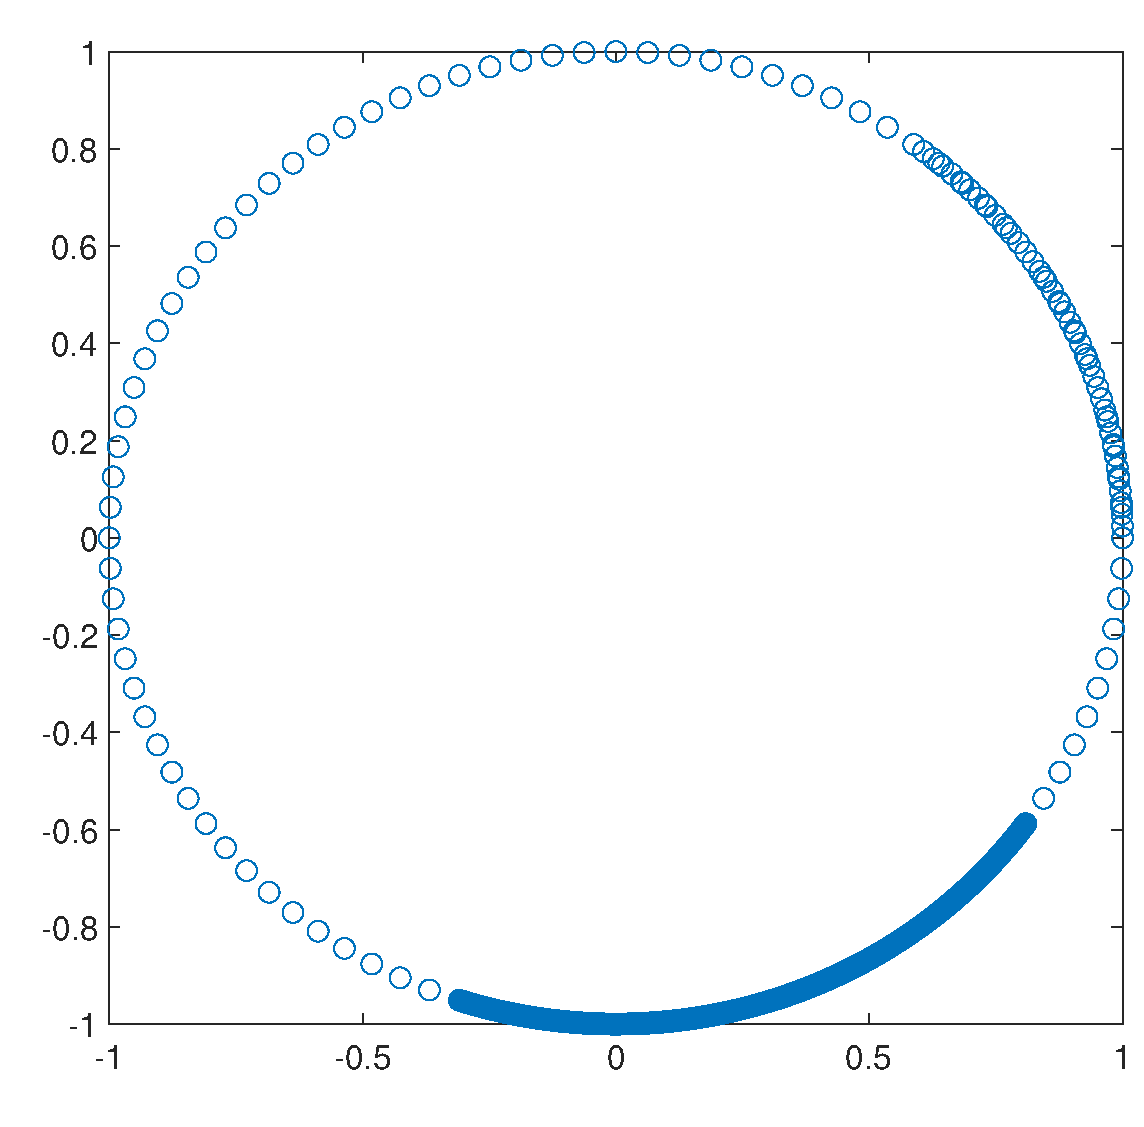
\includegraphics[width = \textwidth]{./figures-1D/nodes.eps}
\subcaption{}
\label{fig:nodes-1D}
\end{subfigure}
\hfill
\begin{subfigure}{0.24\textwidth}
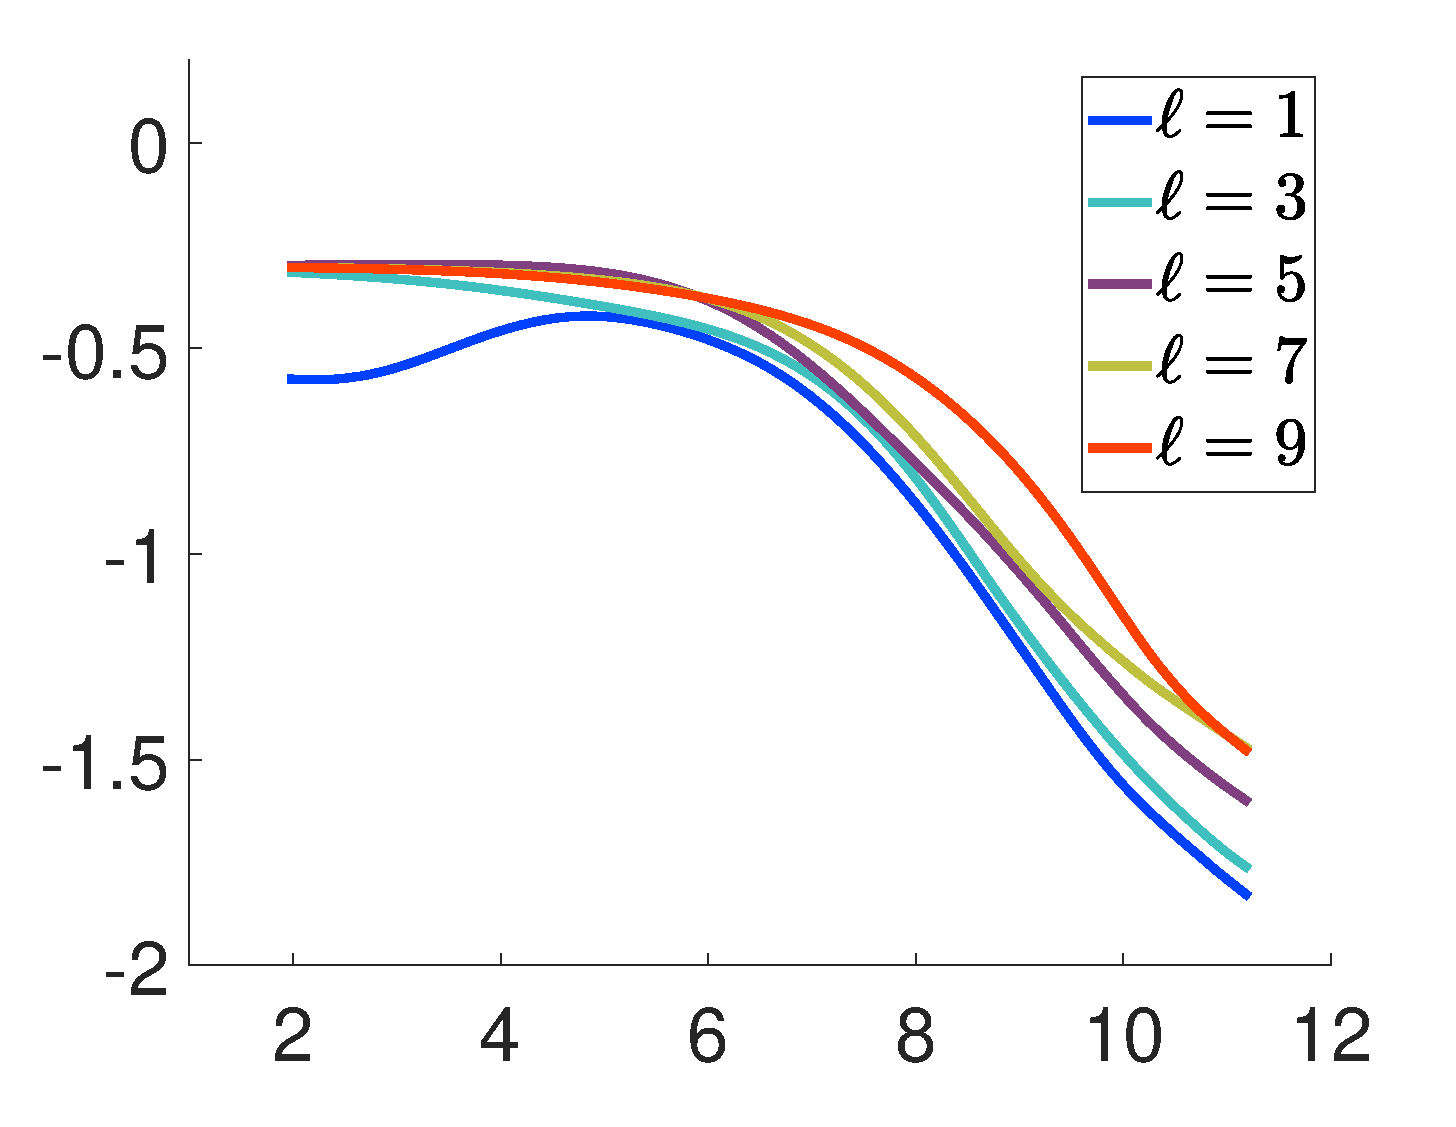
\includegraphics[width = \textwidth]{./figures-1D/uniform_train.eps}
\subcaption{}
\label{fig:uniform_train-1D}
\end{subfigure}
\hfill
\begin{subfigure}{0.24\textwidth}
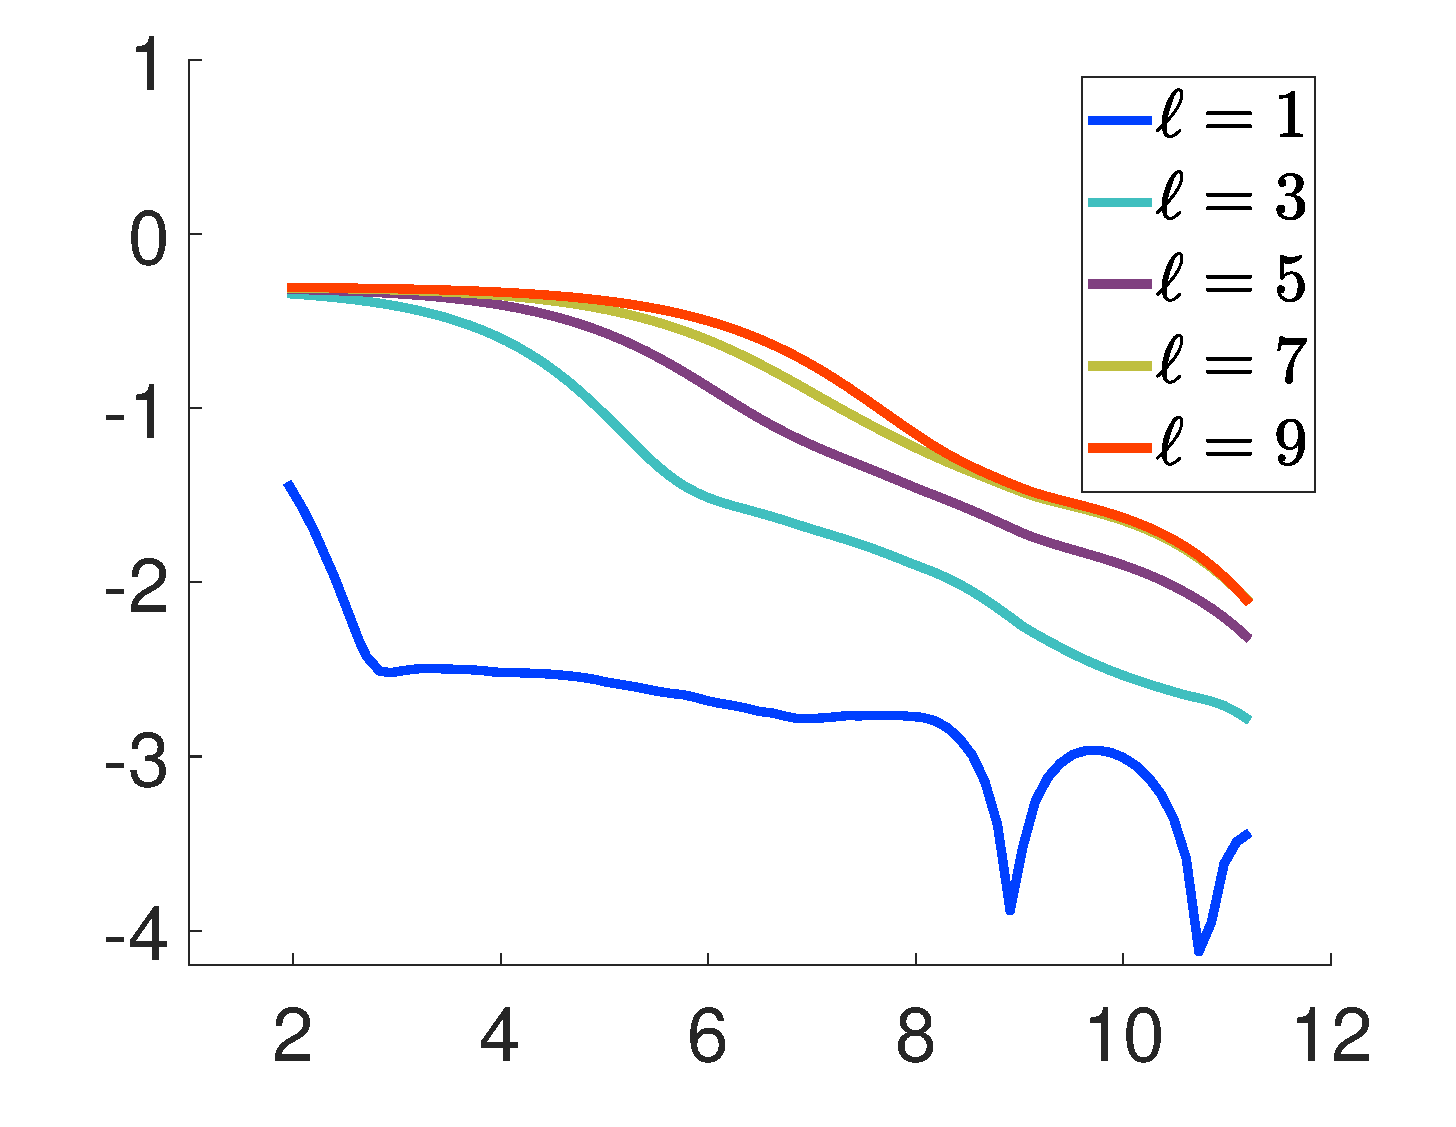
\includegraphics[width = \textwidth]{./figures-1D/weighted_train.eps}
\subcaption{}
\label{fig:weighted_train-1D}
\end{subfigure}
\hfill
\begin{subfigure}{0.24\textwidth}
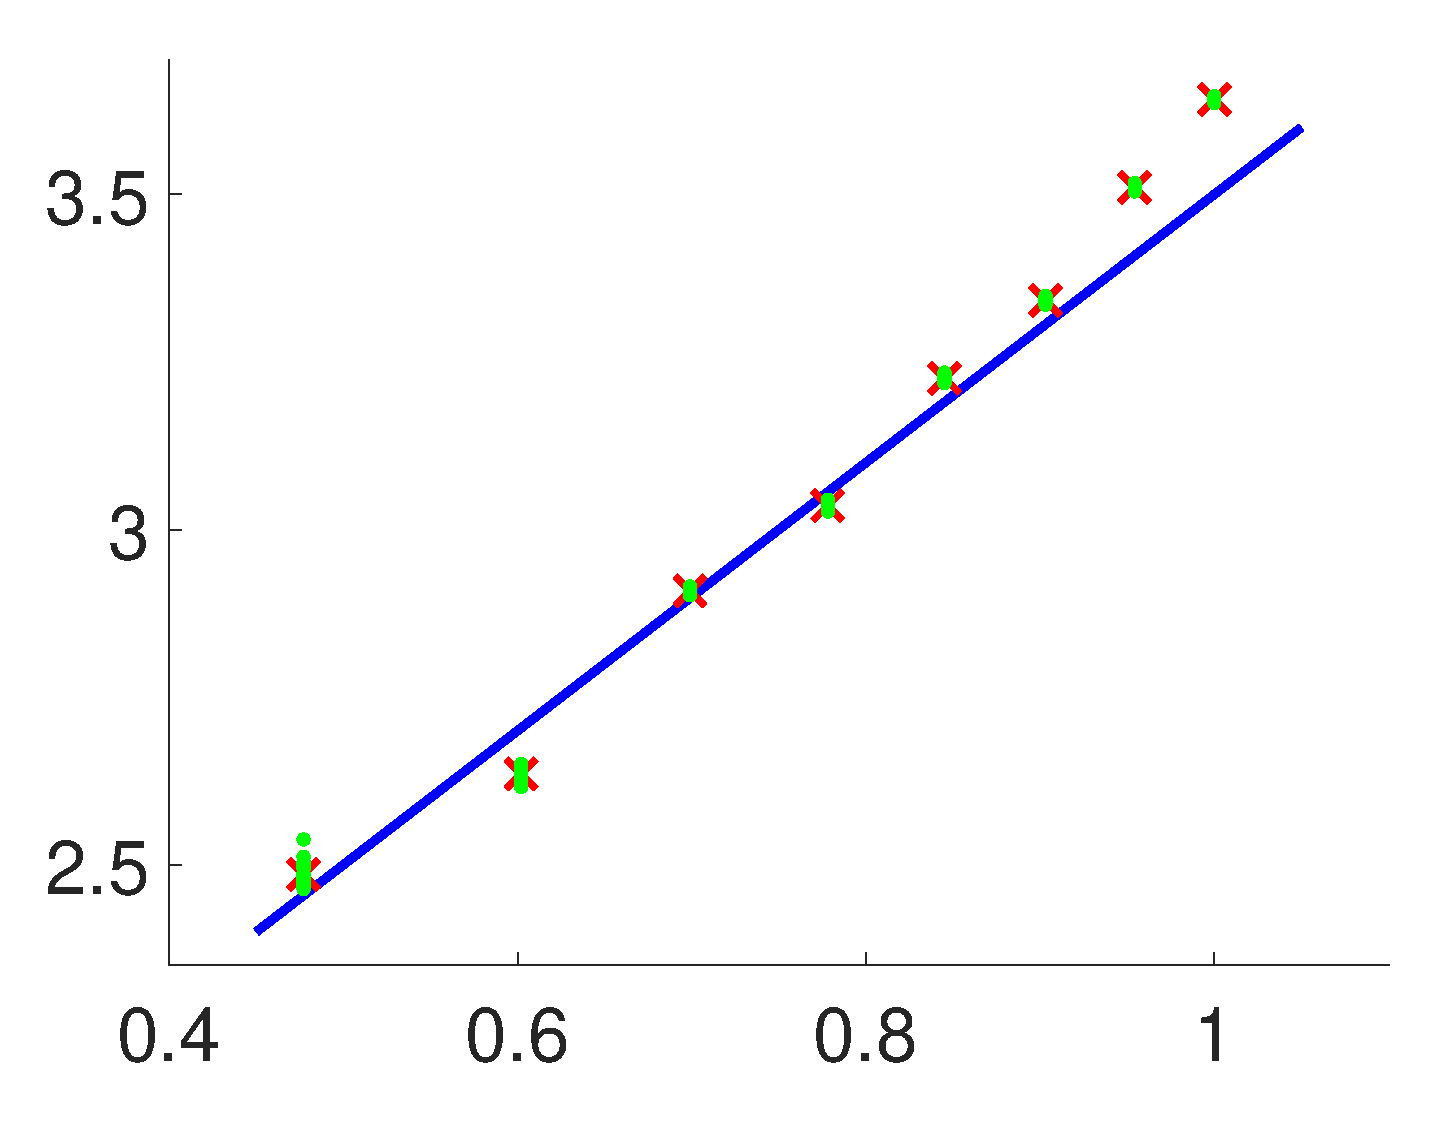
\includegraphics[width = \textwidth]{./figures-1D/iterations.eps}
\subcaption{}
\label{fig:iterations-1D}
\end{subfigure}
\caption{(\subref{fig:nodes-1D}): The distribution of the training data. (\subref{fig:uniform_train-1D}): The change of frequency loss against the number of iterations for $\ell^2$-loss-based training, where $k$ is the frequency and both axes are on the log scale.~(\subref{fig:weighted_train-1D}): The change of frequency loss against the number of iterations for $L^2$-loss-based training, where $k$ is the frequency and both axes are on the log scale.~(\subref{fig:iterations-1D}): The number of iterations needed to achieve a $5.0$ unnormalized $L^2$-loss in learning $\sin(kx)$ for $k = 3, \ldots, 10$ with the weighted loss function. The $x$-axis corresponds to $\ln(k)$ and the $y$-axis is the natural log of the number of iterations. The red crosses correspond to multiple random initializations, the green dots correspond to the average, and the blue line is a reference line of slope $2$ corresponding to the theoretical rate (see~\cite{basri}).}
\label{fig:weighted-1D}
\end{figure}
}



\begin{figure}
\centering
\begin{minipage}{.32\textwidth}
%\begin{overpic}[width=\textwidth]{figures-1D/supplement_minus1} 
\begin{overpic}[width=\textwidth]{figures-1D/Fig5sm1} 
\put(0,30) {\rotatebox{90}{loss}}
\put(40,-2) {epochs}
\end{overpic} 
\end{minipage} 
\begin{minipage}{.32\textwidth}
%\begin{overpic}[width=\textwidth]{figures-1D/supplement_0} 
\begin{overpic}[width=\textwidth]{figures-1D/Fig5s0} 
\put(0,30) {\rotatebox{90}{loss}}
\put(40,-2) {epochs}
\end{overpic} 
\end{minipage}
\begin{minipage}{.32\textwidth}
%\begin{overpic}[width=\textwidth]{figures-1D/supplement_1} 
\begin{overpic}[width=\textwidth]{figures-1D/Fig5s1} 
\put(0,30) {\rotatebox{90}{loss}}
\put(40,-2) {epochs}
\end{overpic} 
\end{minipage}
\caption{Frequency loss for $\ell=3$ (blue), $\ell=5$ (red), and $\ell=9$ (yellow) based on the squared $H^s$ norm as the loss function. Left: $s=-1$; Middle: $s = 0$; Right: $s=1$. The error bars are generated using the results obtained by executions with thirty different random seeds. In the left figure, the result of one of the thirty executions is omitted because the NN is trapped by a local minimizer that is not a global one, making the NN not converge to the target function. \label{fig:sobolev-1D}}
\end{figure} 


\subsection{Learning spherical harmonics on the unit sphere}
%\red{the training point (e.g., $x_i$'s) are not given here}
In~\cref{sec:test2}, we train a NN with data derived from sampling function defined on $\mathbb{S}^2$ at nonuniform points. The training data is a maximum determinant set of 2500 points that comes from the so-called ``spherepts'' dataset~\citep{wright2015}. In this experiment, the target function is
\[
    g(\mathbf{x}) = \sum_{\ell=1}^{15} Y_{2\ell,0}(\mathbf{x}),
\]
where $Y_{2\ell, 0}$ is the normalized zonal spherical harmonic function of degree $2\ell$. Therefore, the spherical harmonic coefficients of $g$ defined in~\cref{eq:g_lp} satisfy $\hat{g}_{\ell,p} = 1$ if $p = 0$ and $\ell = 2, 4, \ldots, 30$, and $\hat{g}_{\ell,p} = 0$ otherwise. We then train an NN with the squared $H^s$ norm as the loss function (see~\cref{eq.sobolevloss}) for $s= -1, 0, 2.5$. By~\Cref{thm.sobconvergence}, we need $\lmax \geq L = 30$. We set $\lmax = 40$ in~\cref{eq.sobolevloss}, assuming that the bandwidth $L$ is not known a priori.
%\red{This doesn't make much sense. You constructed $g$ so you know its bandwidth. Why is this an assumption? Instead, I think this is because you need to decide our to discretize the $H^s$ norm in the loss function} 
We observe frequency biasing in this experiment by considering $|\widehat{\NN}_{\ell,p} - \hat{g}_{\ell,p}|$ after each epoch for $\ell = 4,10,20$. We confirm that low frequencies of $g$ are captured earlier in training than high frequencies when $s = -1$ and $s = 0$ (see~\Cref{fig:2D}, left and middle), and that this frequency biasing phenomena can be counterbalanced by taking $s = 2.5$ (see~\Cref{fig:2D}, right).

%The frequency loss of the residual is defined as $|\hat z_{\ell, p}| = |\widehat{\NN}_{\ell,p} - \hat{g}_{\ell,p}|$. We plot $|\hat z_{\ell, 0}|$ for different $\ell$ in~\Cref{fig:2D}.

\subsection{Test on Autoencoder}
Autoencoders can be used as a generative model to randomly generate new data that is similar to the training data. In this experiment, we use Sobolev-based norms to improve NN training for producing new images of digits that match the MNIST dataset.  In our final experiment, we use the same autoencoder architecture as in~\citep{autoencoder}, except we train the autoencoder with a different loss function (see~\cref{sec:test3}). 

Here, for training images $\{\mathbf{x}_i\}$, a standard loss function can be 
\[
    \Phi(\mathbf{W}) = \frac{1}{2}\int \text{dist} ( \mathcal{N}(\mathbf{x}) , \mathbf{x} ) d\mu(\mathbf{x}) \approx \frac{1}{2n} \sum_{i=1}^n \text{dist} ( \mathcal{N}(\mathbf{x}_i) , \mathbf{x}_i ),
\]
where $\mu$ is the distribution of the training images and $\text{dist} ( \mathcal{N}(\mathbf{x}_i) , \mathbf{x}_i )$ is a distance between the output of the NN given by $\mathcal{N}(\mathbf{x})$ and the image $\mathbf{x}$. %Instead we consider the $L^2$ loss function given by (see~\cref{eq:framework2})
%\[
   %\widetilde \Phi(\mathbf{W}) = \frac{1}{2} \int \text{dist} ( \mathcal{N}(\mathbf{x}) , \mathbf{x} ) d\mathbf{x}  \approx \frac{1}{2} \sum_{i=1}^n c_i \, \text{dist} ( \mathcal{N}(\mathbf{x}_i) , \mathbf{x}_i ),
%\]
%where $\{c_i\}$ are the quadrature weights chosen for the images $\{\mathbf{x}_i\}$. \red{Say how we compute the quadrature weights.}
We select the distance metric to measure the difference between $\mathcal{N}(\mathbf{x})$ and $\mathbf{x}$ as
\begin{equation}
\Phi(\mathbf{W}) =  \frac{1}{2n} \sum_{i=1}^n \|  \mathcal{N}(\mathbf{x}_i)- \mathbf{x}_i \|_F^2 , 
\label{eq:dist} 
\end{equation} 
where $\|\cdot \|_F$ denotes the matrix Frobenius norm. The distance metric in~\cref{eq:dist} can be viewed as  a discretization of the continuous $L^2$ norm. That is, if one imagines generating a continuous function $x: [0,1]^2 \rightarrow [0,\infty)$ that interpolates an image as well as a function that interpolates the NN, then 
\begin{equation*}
  \frac{1}{N_{\text{pixel}}}\|\mathcal{N}(\mathbf{x})- \mathbf{x} \|_F^2 \approx \iint | \mathcal{N}(x) (y_1, y_2) - x(y_1,y_2)|^2 dy_1 dy_2 = \|\mathcal{N}(x) - x\|_{L^2}^2,
\end{equation*}
where $N_{\text{pixel}}$ is the total number of pixels of the image $\mathbf{x}$. In this continuous viewpoint, the $H^s$ norm is given by (assuming that the continuous interpolating functions $x$ and $\mathcal{N}(x)$ are constructed with periodic boundary conditions)
\begin{equation}\label{eq.sobolevpicture}
    \| \mathcal{N}(x) - x \|^2_{H^s} = \int (1+|\xi|^2)^s | \widehat {\mathcal{N}(x)}(\xi) - \widehat{x}(\xi) |^2 d\xi \approx   \| \mathbf{S}_s \circ \left(\mathbf{F}_l \left( \mathcal{N}(\mathbf{x})- \mathbf{x}\right) \mathbf{F}_r^\top\right) \|_F^2,
\end{equation}
%where the matrix $\mathbf{J}_s$ incorporates the discrete Fourier transform and the $H^s$ norm natural frequency scaling $(1+|\xi|^2)^s$.
where $\mathbf{F}_l, \mathbf{F}_r$ are the left and right 2D-DFT matrices, respectively, $(S_s)_{j\ell} = (1+j^2+\ell^2)^{s/2}$, and `$\circ$' is the Hadamard product. Hence, if we define $\text{vec}(\mathbf{A})$ to be the vector obtained by reshaping a matrix $\mathbf{A}$ using the column major order, then we have
\begin{equation*}
    \| \mathbf{S}_s \circ \left(\mathbf{F}_l \left( \mathcal{N}(\mathbf{x})- \mathbf{x}\right) \mathbf{F}_r^\top\right) \|_F^2 = \norm{\text{diag}(\text{vec}(\mathbf{S}_s)) (\mathbf{F}_r \otimes \mathbf{F}_l) \text{vec}(\mathcal{N}(\mathbf{x})- \mathbf{x})}^2_2,
\end{equation*}
where $\otimes$ is the Kronecker product of two matrices. Setting $\mathbf{J}_s = \text{diag}(\text{vec}(\mathbf{S}_s)) (\mathbf{F}_r \otimes \mathbf{F}_l)$, the loss function in our NN training can be written as
%\red{Give the exact form of $\mathbf{J}_s$.}
\begin{equation} 
    \Phi_s(\mathbf{W}) = \frac{1}{2n} \sum_{i=1}^n \| \mathbf{J}_s \text{vec}\left(\mathcal{N}(\mathbf{x}_i)- \mathbf{x}_i\right) \|_2^2 = \frac{1}{2n} (\mathbf{u} - \mathbf{y})^\top (\mathbf{I} \otimes \mathbf{J}_s^\top \mathbf{J}_s) (\mathbf{u} - \mathbf{y}),
\label{eq:finalloss} 
\end{equation}
where $\mathbf{I}$ is the $n$-by-$n$ identity matrix and $\mathbf{u}, \mathbf{y}$ are the vectors of length $n \times N_{\text{pixel}}$ given by $\mathbf{u} = (\text{vec}(\mathcal{N}(\mathbf{x}_1))^\top, \ldots, \text{vec}(\mathcal{N}(\mathbf{x}_n))^\top)^\top$ and $\mathbf{y} = (\text{vec}(\mathbf{x}_1)^\top, \ldots, \text{vec}(\mathbf{x}_n)^\top)^\top$. Hence, the discrete NTK matrix is given by $n^{-1}\mathbf{H}^\infty (\mathbf{I} \otimes \mathbf{J}_s^\top \mathbf{J}_s)$, where the $(i,j)$th sub-block is $\mathbf{H}^\infty_{ij} = \big \langle \frac{\partial \text{vec}(\mathcal{N}(\mathbf{x}_i;\mathbf{W})) }{\partial \mathbf{W}},\frac{\partial \text{vec}(\mathcal{N}(\mathbf{x}_j;\mathbf{W}))}{\partial \mathbf{W}}  \big \rangle$ for $i, j = 1, \ldots, n$. Here, $\big \langle \frac{\partial \text{vec}(\mathcal{N}(\mathbf{x}_i;\mathbf{W})) }{\partial \mathbf{W}},\frac{\partial \text{vec}(\mathcal{N}(\mathbf{x}_j;\mathbf{W}))}{\partial \mathbf{W}}  \big \rangle$ is interpreted as the $N_{\text{pixel}}$-by-$N_{\text{pixel}}$ matrix whose $(i',j')$th entry is $\big \langle \frac{\partial [\text{vec}(\mathcal{N}(\mathbf{x}_i;\mathbf{W}))_{i'}] }{\partial \mathbf{W}},\frac{\partial [\text{vec}(\mathcal{N}(\mathbf{x}_j;\mathbf{W}))_{j'}]}{\partial \mathbf{W}}  \big \rangle$. This means that the frequency biasing behavior during NN training is directly affected by the choice of $s$. We remark that while~\cref{eq:finalloss} is a mathematically equivalent expression for the loss function that allows us to easily express the NTK, in practice, we implement the loss function based on~\cref{eq.sobolevpicture} using a 2D FFT protocol.

We use the same autoencoder architecture as in~\citep{autoencoder}, except with the loss function in~\cref{eq:finalloss} for $s = -1, 0, 1$. \revise{We train the autoencoder using mini-batch gradient descent with batch size equal to $256$.} We first pollute the training images with low-frequency noise and train the NN, hoping that the trained NN will act as filter for the noise. We see that training the NN with~\cref{eq:finalloss} for $s = 1$ gives us the best results due to the high-frequency biasing induced by the choice of the loss function. Although $\mathbf{H}^\infty$ is low frequency biasing, the high-frequency biasing of $\mathbf{J}_s^\top \mathbf{J}_s$ dominates for sufficiently large $s$. In that case, the low-frequency noise barely changes the training in the earlier epochs as the low-frequency components of the residual correspond to small eigenvalues of $\mathbf{H}^\infty (\mathbf{I} \otimes \mathbf{J}_s^\top \mathbf{J}_s)$.  Similar results are discussed in~\citep{engquist2020quadratic} and \citep{yang2021implicit} in the inverse problem and image processing contexts, respectively.

The opposite phenomenon occurs when we add high-frequency noise (see~\Cref{fig:autoencoder}, bottom row). Since $\mathbf{H}^\infty$ by itself makes the NN training procedure bias towards low-frequencies, the output for $s=0$ does already filter high-frequency noise. Since $\mathbf{J}_s^\top \mathbf{J}_s$ for $s<0$ further biases towards low-frequencies, one can obtain better high-frequency filters. We observe that the best denoising results for the autoencoder comes from selecting $s=-1$ (see~\Cref{fig:autoencoder}, bottom row).

\section{Computation of Quadrature Weights}\label{sec:computeweight}

\revise{
In practice, the training dataset usually does not come with a carefully designed quadrature rule. Hence, we inevitably need to compute a set of quadrature weights before training the NN. In this section, we briefly discuss methods for computing positive quadrature weights.}

\revise{Given a set of points $\{\mathbf{x}_i\}_{i=1}^n$ on $\sS^{d-1}$, we wish to construct a quadrature rule so that
\begin{equation*}
    I_n(f) := \sum_{i=1}^n c_i f(\mathbf{x}_i) \approx \int_{\sS^{d-1}} f(\mathbf{x}) d\mathbf{x}
\end{equation*}
for sufficiently smooth $f$, where $c_i > 0$ are positive quadrature weights. One approach that could give us a very accurate quadrature rule is to guarantee that
\begin{equation}\label{eq.exactquadrule}
    I_n(f) = \int_{\sS^{d-1}} f(\mathbf{x}) d\mathbf{x}, \qquad f \in \Pi_\ell^d,
\end{equation}
where $\text{dim}(\Pi_\ell^d) \leq n$. The one-dimensional case of such quadrature rules was studied in~\citep{austin2017trig,yu2022stability} and the general higher-dimensional case was analyzed in~\citep{mhaskar,dai}. Given any dataset $\{\mathbf{x}_i\}_{i=1}^n$ and $\ell$ so that $\text{dim}(\Pi_\ell^d) \leq n$, one cannot guarantee the existence of a positive quadrature rule satisfying~\cref{eq.exactquadrule}~\citep{mhaskar,dai}, even when the distribution of $\{\mathbf{x}_i\}_{i=1}^n$ is very regular~\citep{yu2022stability}. On the other hand, by choosing $\ell$ to be small, we can eventually find an $\ell$ for which~\cref{eq.exactquadrule} holds. When such a positive quadrature rule exists,~\cite{mhaskar} proposed to solve the following feasible constrained quadratic program
\begin{equation*}
\begin{aligned}
\min_{c_i} \quad & \sum_{i=1}^n c_i^2\\
\textrm{s.t.} \quad & c_i > 0 \quad \forall 1 \leq i \leq n,\\
  & \sum_{i=1}^n c_i Y_{j,p}(\mathbf{x}_i) = \int_{\sS^{d-1}} Y_{j,p}(\mathbf{x}) d\mathbf{x} \quad \forall 0 \leq j \leq \ell, 1 \leq p \leq N(d,j).
\end{aligned}
\end{equation*}
}

\revise{
While~\cref{eq.exactquadrule} gives us guarantee on the accuracy of the quadrature rule (provided $\ell$ is not too small), it is not always practical to compute the quadrature weights in this way. Indeed, if $d$ is large, then we need tremendous amount of points to guarantee that $\text{dim}(\Pi_\ell^d) \leq n$ even for a small $\ell$. Also, if we have too many data points, then the quadratic program can get infeasible to solve. Hence, we need some other methods for computing quadrature weights that, albeit less accurate, can be applied more cheaply to general datasets. One of the many possible approaches is to do kernel density estimation~\citep{rosenblatt1956remarks,parzen1962estimation}. To do so, we fix a positive kernel $\mathcal{K}(\mathbf{x},\mathbf{y}) = \mathcal{K}(\arccos(\mathbf{x}^\top \mathbf{y}))$ defined on $\sS^{d-1} \times \sS^{d-1}$. A common choice of $\mathcal{K}$ can be the Gaussian density function of standard deviation $1$ centered at $0$. For each $h > 0$, we then define a function $p_h$ on $\sS^{d-1}$ by
\begin{equation*}
    p_h(\mathbf{x}) = \sum_{i=1}^n \mathcal{K}\left(\frac{\arccos(\mathbf{x}^\top \mathbf{x}_i)}{h}\right).
\end{equation*}
The bandwidth $h$ is a hyperparameter, and with an appropriate $h$, the function $p_h$ is an (unnormalized) estimate of the density function of the distribution of nodes. Hence, by setting
\begin{equation}
    c_i = A_d \frac{p_h^{-1}(\mathbf{x}_i)}{\sum_{j=1}^n p_h^{-1}(\mathbf{x}_j)},
\end{equation}
we obtain a positive quadrature rule that approximates the integral of smooth functions on $\sS^{d-1}$.
}



% \bibliographystyle{plainnat}
% \bibliography{references}

% \end{document}